% vim: set tw=78 tabstop=4 shiftwidth=4 aw ai:
\documentclass{beamer}

\usepackage[utf8x]{inputenc}		% diacritice
\usepackage[romanian]{babel}
\usepackage{color}			% highlight
\usepackage{alltt}			% highlight
\usepackage{minted}

% highlight; comment this out in case you don't input code source files
\usepackage{code/highlight}		% highlight

\usepackage{hyperref}			% folosiți \url{http://...}
					% sau \href{http://...}{Nume Link}
\usepackage{verbatim}

\usepackage{subcaption}

\def\code#1{\texttt{#1}}

\mode<presentation>
{ \usetheme{Berlin} }

% Încărcăm simbolurilor Unicode românești în titlu și primele pagini
\PreloadUnicodePage{200}

% Arătăm numărul frame-ului
\newcommand{\frameofframes}{/}
\newcommand{\setframeofframes}[1]{\renewcommand{\frameofframes}{#1}}

\setframeofframes{of}
\makeatletter
\setbeamertemplate{footline}
  {%
    \begin{beamercolorbox}[colsep=1.5pt]{upper separation line foot}
    \end{beamercolorbox}
    \begin{beamercolorbox}[ht=2.5ex,dp=1.125ex,%
      leftskip=.3cm,rightskip=.3cm plus1fil]{author in head/foot}%
      \leavevmode{\usebeamerfont{author in head/foot}\insertshortauthor}%
      \hfill%
      {\usebeamerfont{institute in head/foot}\usebeamercolor[fg]{institute in head/foot}\insertshortinstitute}%
    \end{beamercolorbox}%
    \begin{beamercolorbox}[ht=2.5ex,dp=1.125ex,%
      leftskip=.3cm,rightskip=.3cm plus1fil]{title in head/foot}%
      {\usebeamerfont{title in head/foot}\insertshorttitle}%
      \hfill%
      {\usebeamerfont{frame number}\usebeamercolor[fg]{frame number}\insertframenumber~\frameofframes~\inserttotalframenumber}
    \end{beamercolorbox}%
    \begin{beamercolorbox}[colsep=1.5pt]{lower separation line foot}
    \end{beamercolorbox}
  }
\makeatother

\setbeamertemplate{navigation symbols}{}%remove navigation symbols
\setbeamertemplate{caption}[numbered]

\title[Eliminarea recursivității în programele Java]{Eliminarea recursivității în programele Java}
\subtitle{Sesiunea de licență -- septembrie 2017}
\institute{Facultatea de Automatică și Calculatoare,\\
	Universitatea POLITEHNICA București}
\author[Andrei Silviu Dragnea]{Andrei Silviu Dragnea\\
	Coordonator: Prof. dr. ing. Lorina Negreanu}
\date{11 septembrie 2017}

\begin{document}

% Slide-urile cu mai multe părți sunt marcate cu textul (cont.)
\setbeamertemplate{frametitle continuation}[from second]

% Arătăm numărul frame-ului
%\setbeamertemplate{footline}[frame number]

\frame{\titlepage}

\frame{\tableofcontents}

% NB: Secțiunile nu sunt marcate vizual, ci doar apar în cuprins
\section{Context}

% Titlul unui frame se specifică fie în acolade, imediat după \begin{frame},
% fie folosind \frametitle
\begin{frame}{Intellij IDEA plugin}
    \begin{columns}[T]
        \begin{column}{\textwidth}
            \begin{figure}
                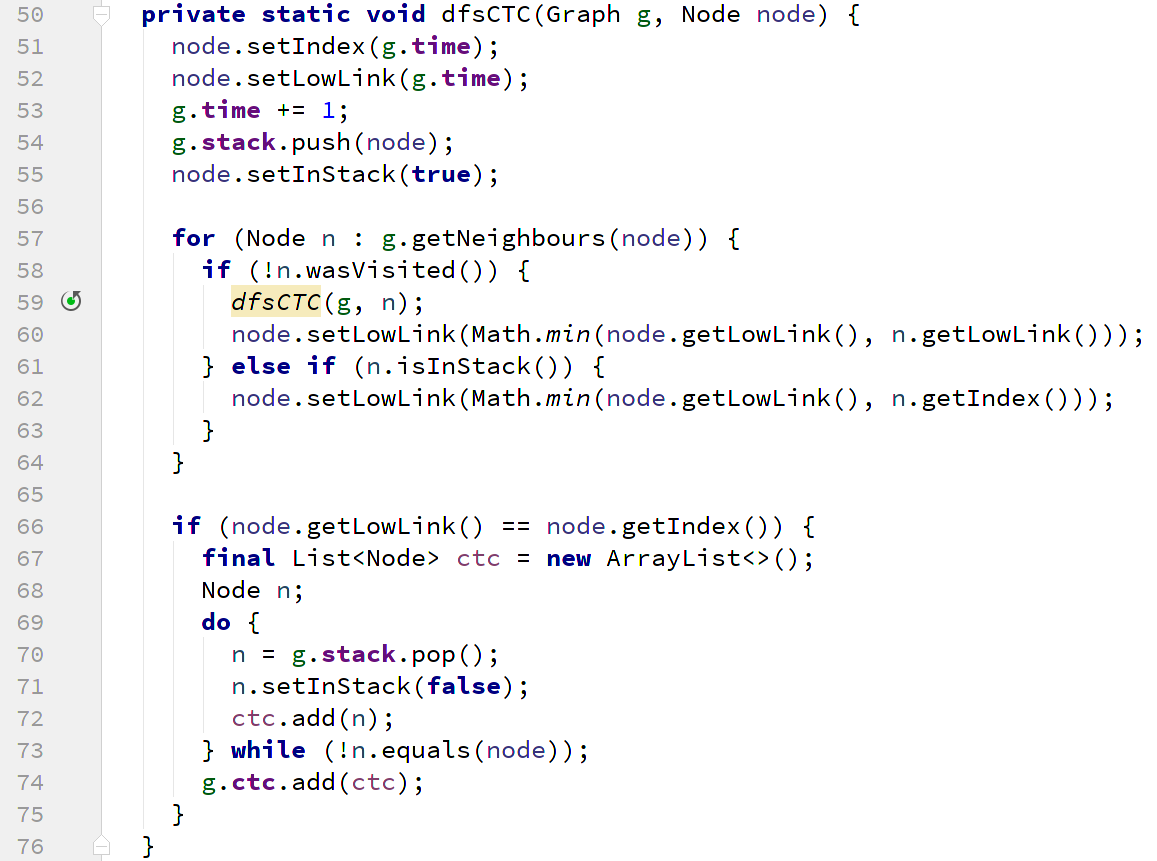
\includegraphics[height=6cm]{img/highlight}
            \end{figure}
        \end{column}
    \end{columns}
\end{frame}

\section{Arhitectură și design}

\begin{frame}{TODO}
	\begin{itemize}
		\item Formulă simplă
			\begin{beamerboxesrounded}[lower=block body,shadow=true]{}
				\texttt{\#define MAX(a, b)   ((a) > (b) ? (a) : (b))}
			\end{beamerboxesrounded}
		\item TODO
	\end{itemize}
\end{frame}

\section{Implementare}

\begin{frame}{Încapsularea instrucțiunilor în blocuri}
    \begin{figure}[htb]
        \makebox[\linewidth][c]{%
        \begin{subfigure}[b]{.6\linewidth}
            \centering
            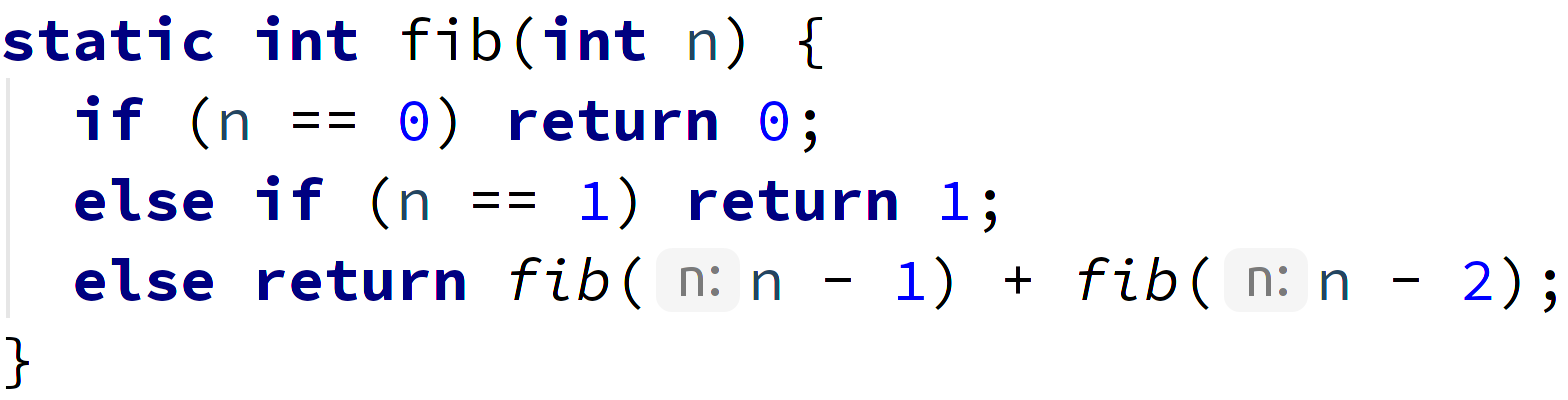
\includegraphics[height=0.6in]{../../../theses/diploma/src/img/replace-single-statements-with-block-statements-before-white.png}
            \caption{Înainte}
        \end{subfigure}%
        \begin{subfigure}[b]{.6\linewidth}
            \centering
            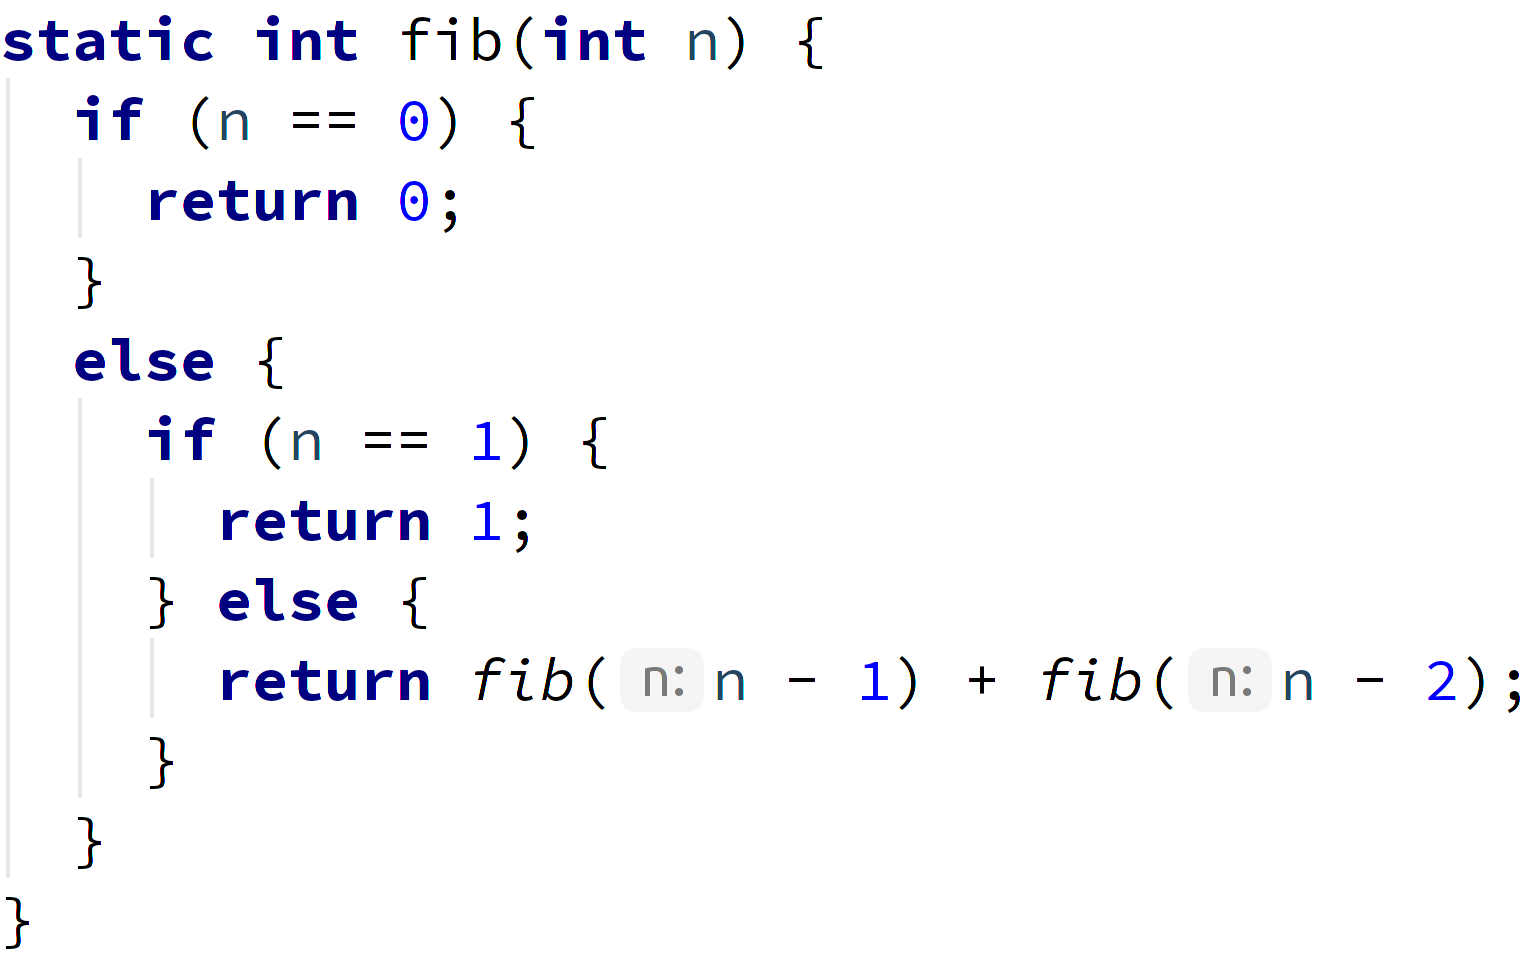
\includegraphics[height=1.44in]{../../../theses/diploma/src/img/replace-single-statements-with-block-statements-after-white.png}
            \caption{După}
        \end{subfigure}%
        }\\
        \caption{Încapsularea instrucțiunilor în blocuri}
    \end{figure}
\end{frame}

\begin{frame}{Expandarea buclelor \code{foreach}}
    \begin{figure}[htb]
        \makebox[\linewidth][c]{%
        \begin{subfigure}[b]{.55\linewidth}
            \centering
            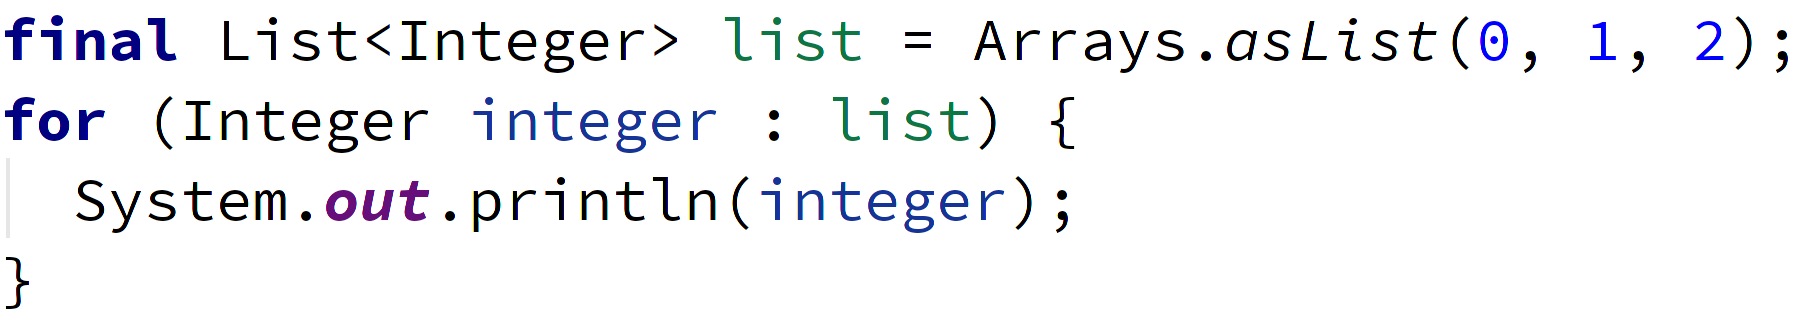
\includegraphics[height=0.4in]{../../../theses/diploma/src/img/foreach-to-iterator-for-before-white.png}
            \caption{Înainte}
        \end{subfigure}%
        \begin{subfigure}[b]{.55\linewidth}
            \centering
            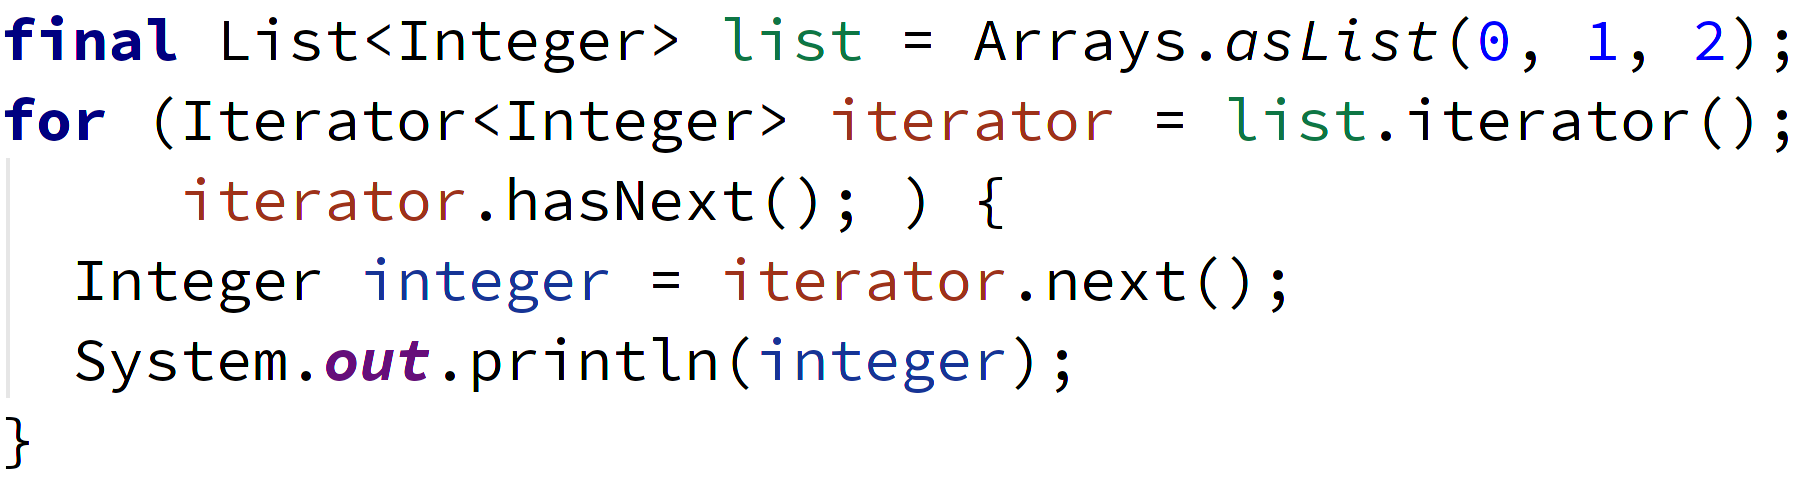
\includegraphics[height=0.6in]{../../../theses/diploma/src/img/foreach-to-iterator-for-after-white.png}
            \caption{După}
        \end{subfigure}%
        }\\
        \caption{Expandarea \code{foreach} bazat pe iterator}
    \end{figure}

    \begin{figure}[htb]
        \makebox[\linewidth][c]{%
        \begin{subfigure}[b]{.55\linewidth}
            \centering
            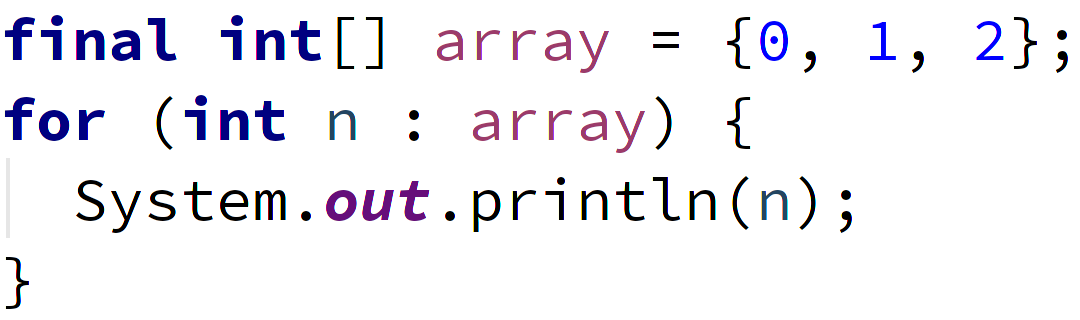
\includegraphics[height=0.4in]{../../../theses/diploma/src/img/foreach-to-indexed-for-before-white.png}
            \caption{Înainte}
        \end{subfigure}%
        \begin{subfigure}[b]{.55\linewidth}
            \centering
            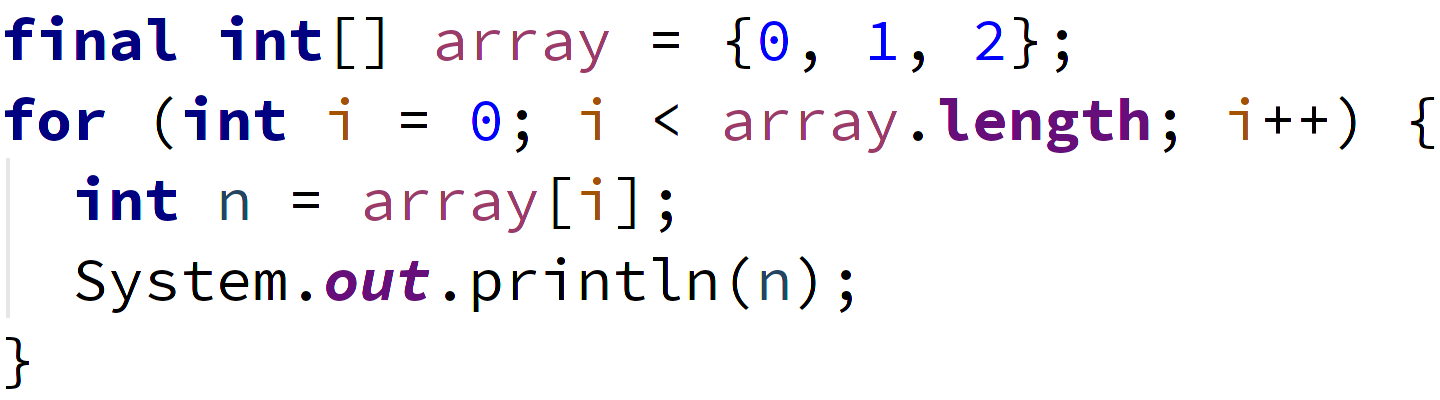
\includegraphics[height=0.5in]{../../../theses/diploma/src/img/foreach-to-indexed-for-after-white.png}
            \caption{După}
        \end{subfigure}%
        }\\
        \caption{Expandarea \code{foreach} bazat pe array}
    \end{figure}
\end{frame}

\begin{frame}{Extragerea apelurilor recursive în instrucțiuni separate}
    \begin{figure}[htb]
        \makebox[\linewidth][c]{%
        \begin{subfigure}[b]{.5\textwidth}
            \centering
            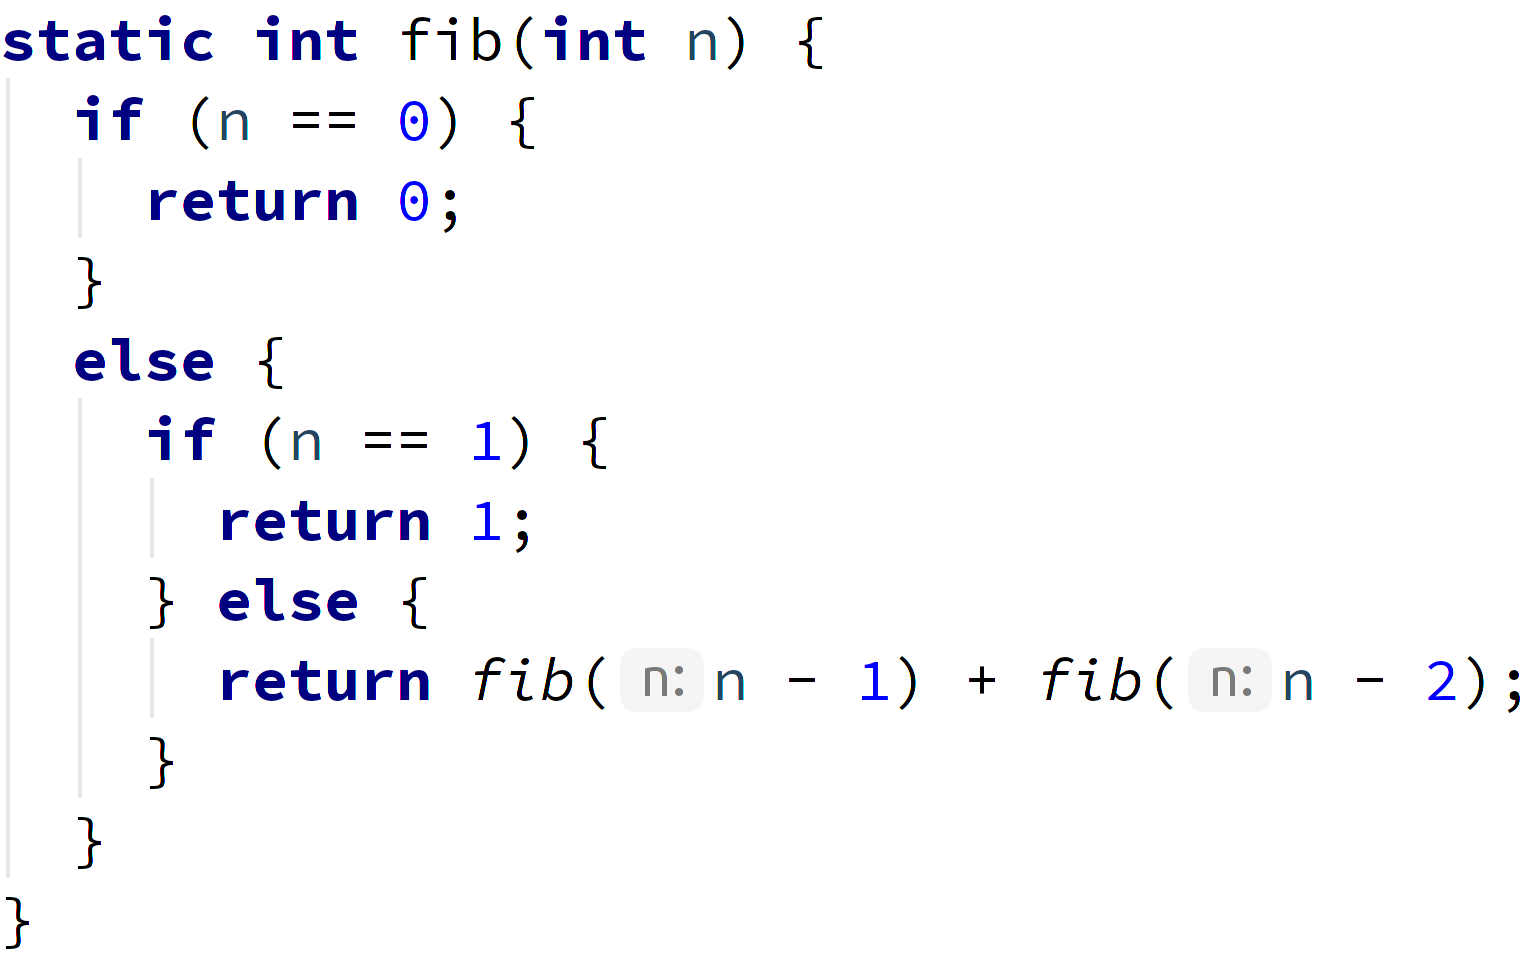
\includegraphics[height=1.44in]{../../../theses/diploma/src/img/replace-single-statements-with-block-statements-after-white.png}
            \caption{Înainte}
        \end{subfigure}%
        \begin{subfigure}[b]{.5\textwidth}
            \centering
            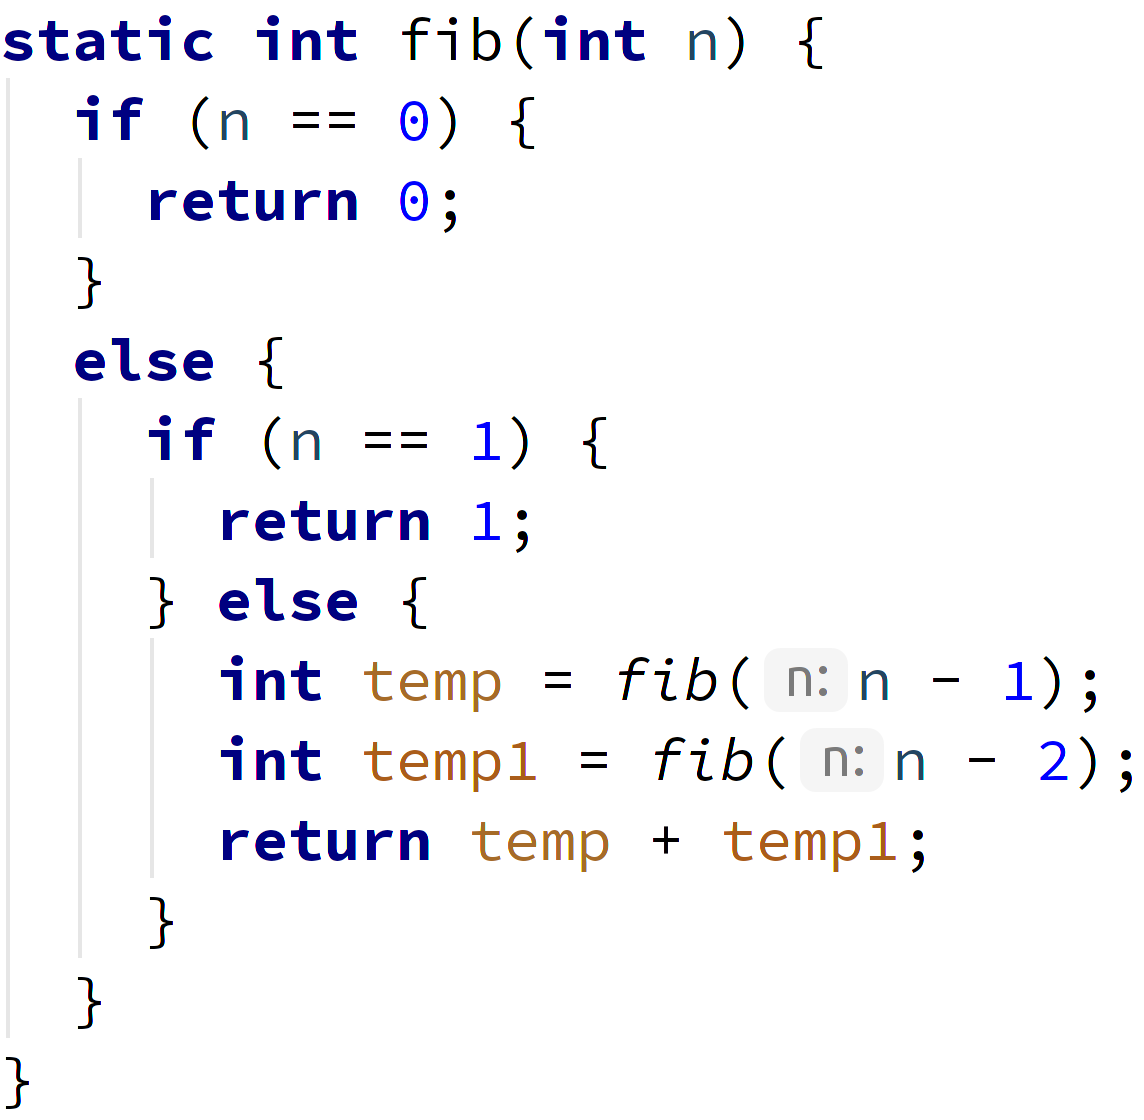
\includegraphics[height=1.68in]{../../../theses/diploma/src/img/extract-after-white.png}
            \caption{După}
        \end{subfigure}%
        }\\
        \caption{Extragerea apelurilor recursive în instrucțiuni separate}
    \end{figure}
\end{frame}

\begin{frame}{Generarea clasei cadru de stivă}
    \begin{figure}[htb]
        \makebox[\linewidth][c]{%
        \begin{subfigure}[b]{.6\textwidth}
            \centering
            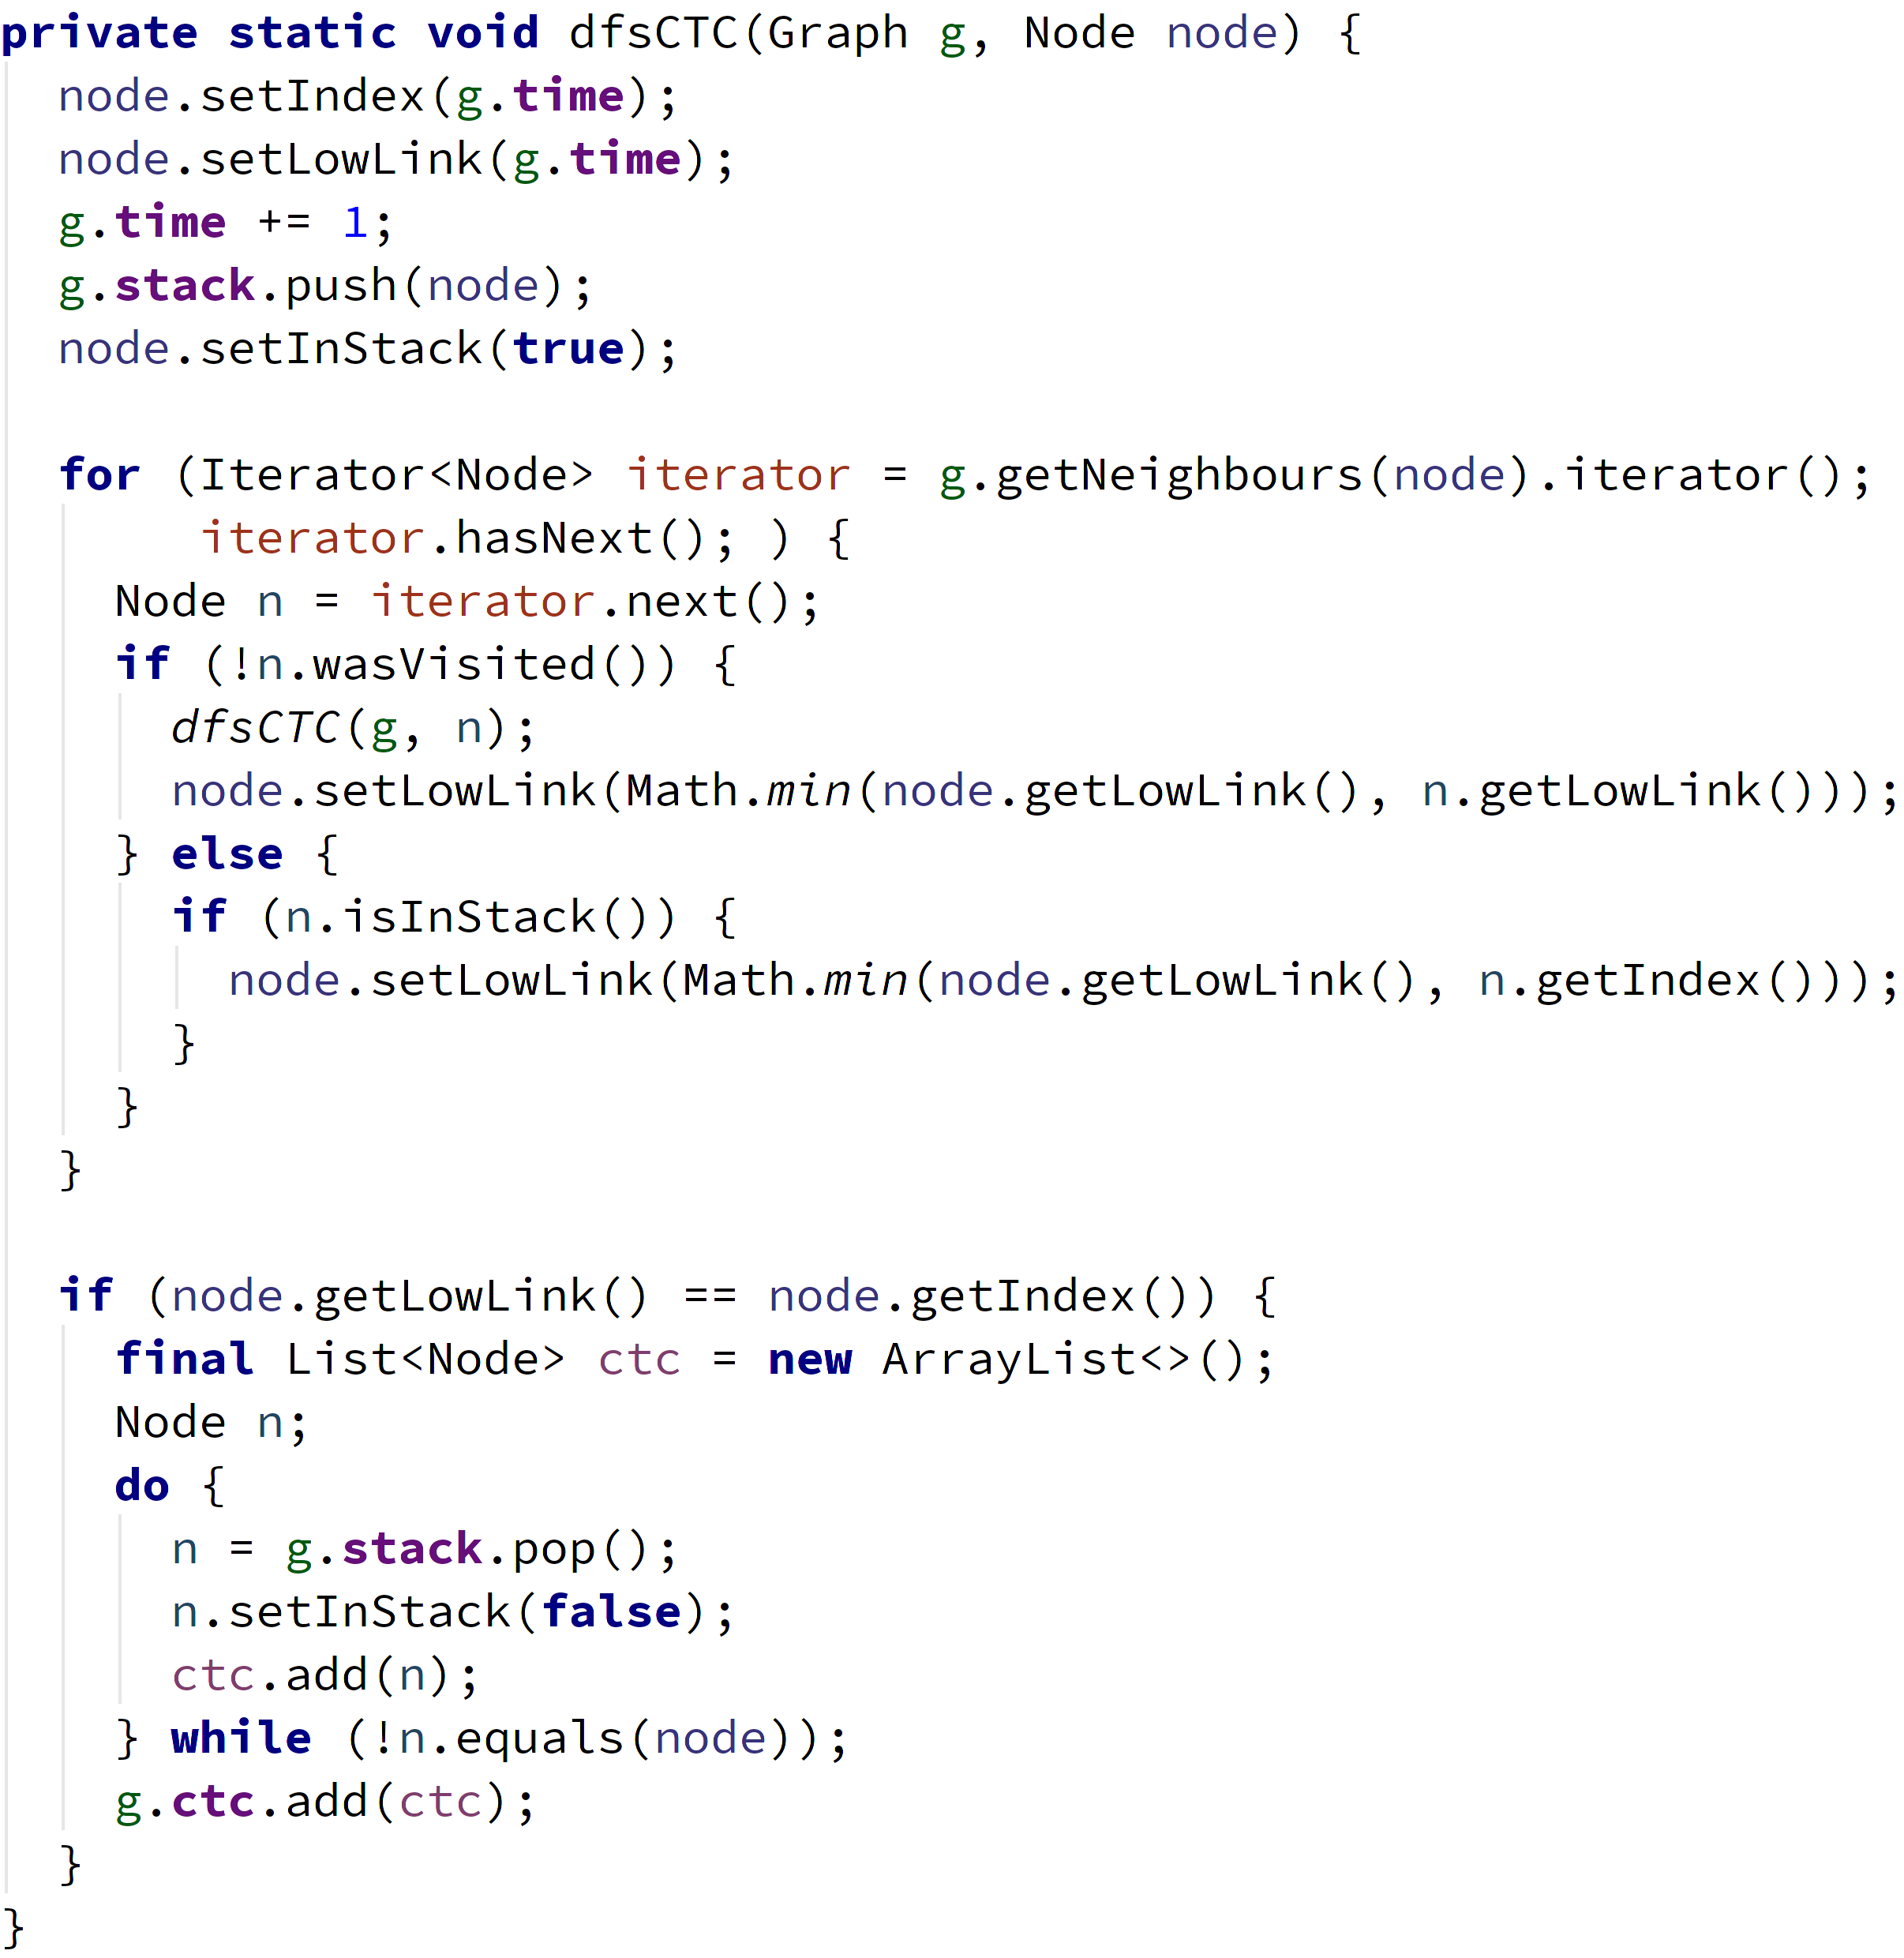
\includegraphics[height=1.75in]{../../../theses/diploma/src/img/add-frame-class-before-white-31.png}
            \caption{Înainte}
        \end{subfigure}%
        \begin{subfigure}[b]{.6\textwidth}
            \centering
            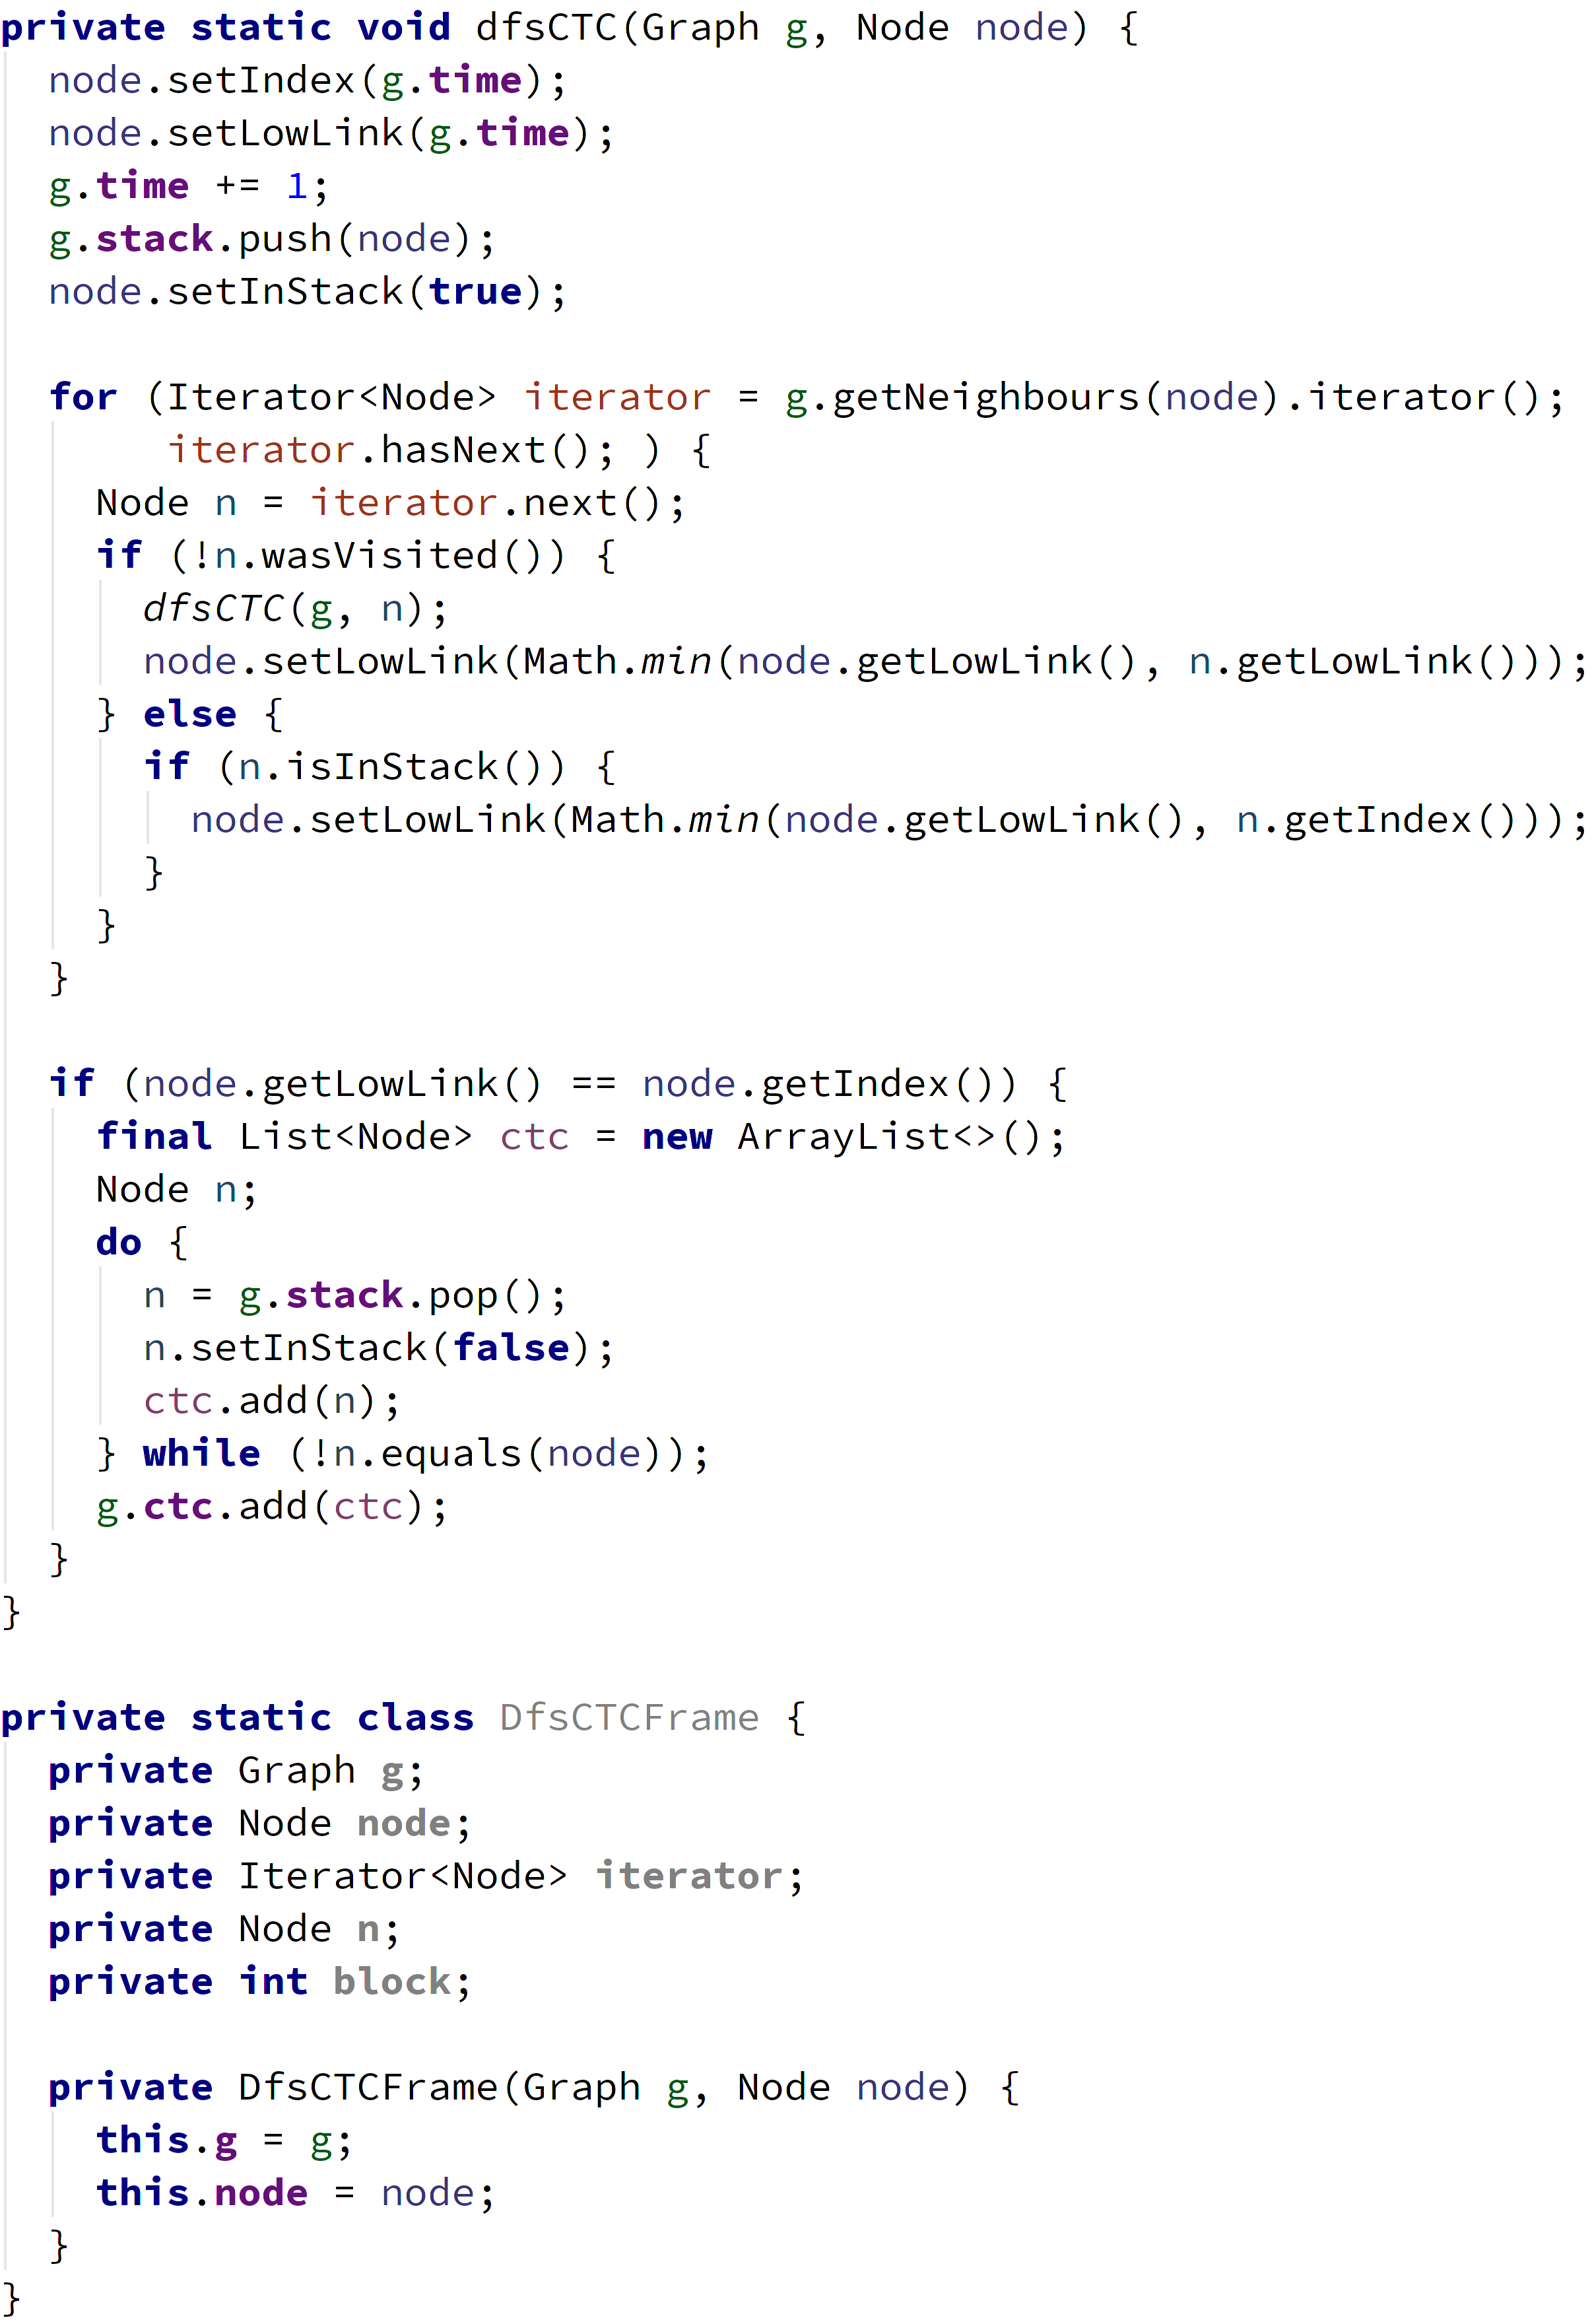
\includegraphics[height=2.484in]{../../../theses/diploma/src/img/add-frame-class-after-white-44.png}
            \caption{După}
        \end{subfigure}%
        }\\
        \caption{Generarea clasei cadru de stivă}
    \end{figure}
\end{frame}

\begin{frame}{Includerea codului metodei în codul auxiliar}
    \begin{figure}[htb]
        \makebox[\linewidth][c]{%
        \begin{subfigure}[b]{.5\textwidth}
            \centering
            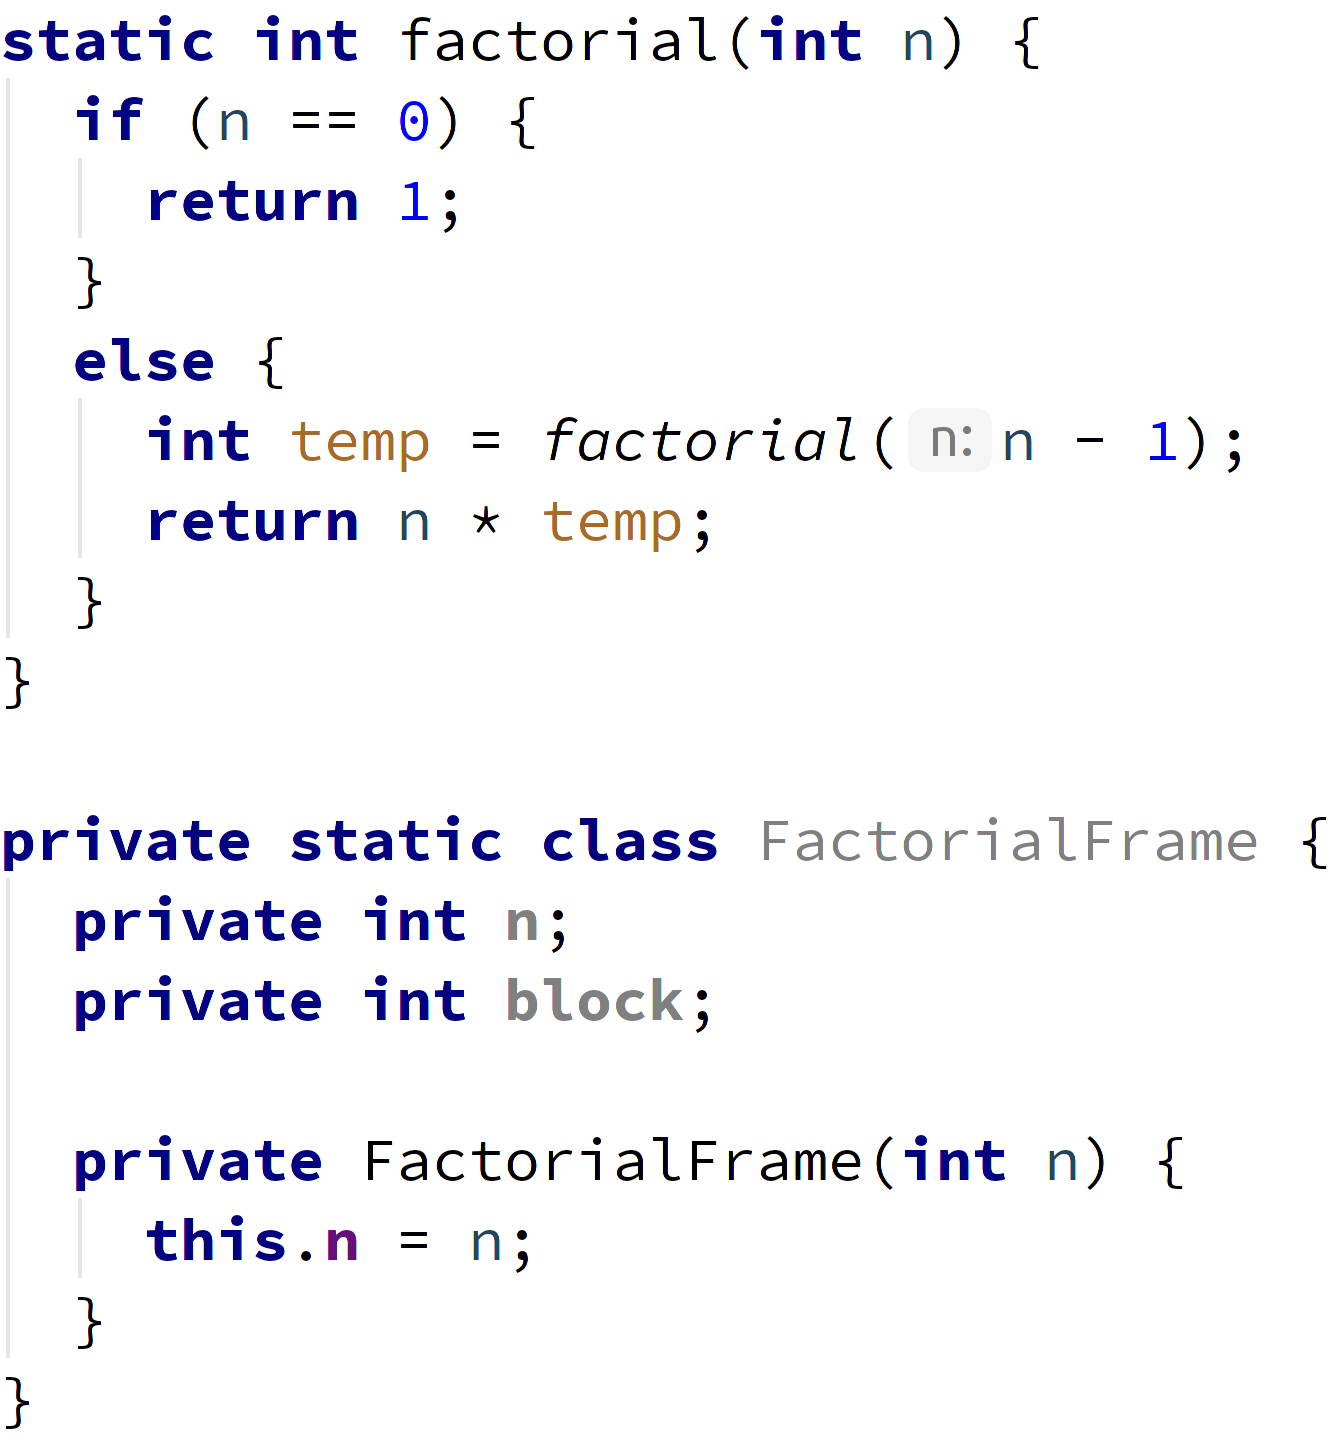
\includegraphics[height=1.7in]{../../../theses/diploma/src/img/incorporate-before-white-18.png}
            \caption{Înainte}
        \end{subfigure}%
        \begin{subfigure}[b]{.5\textwidth}
            \centering
            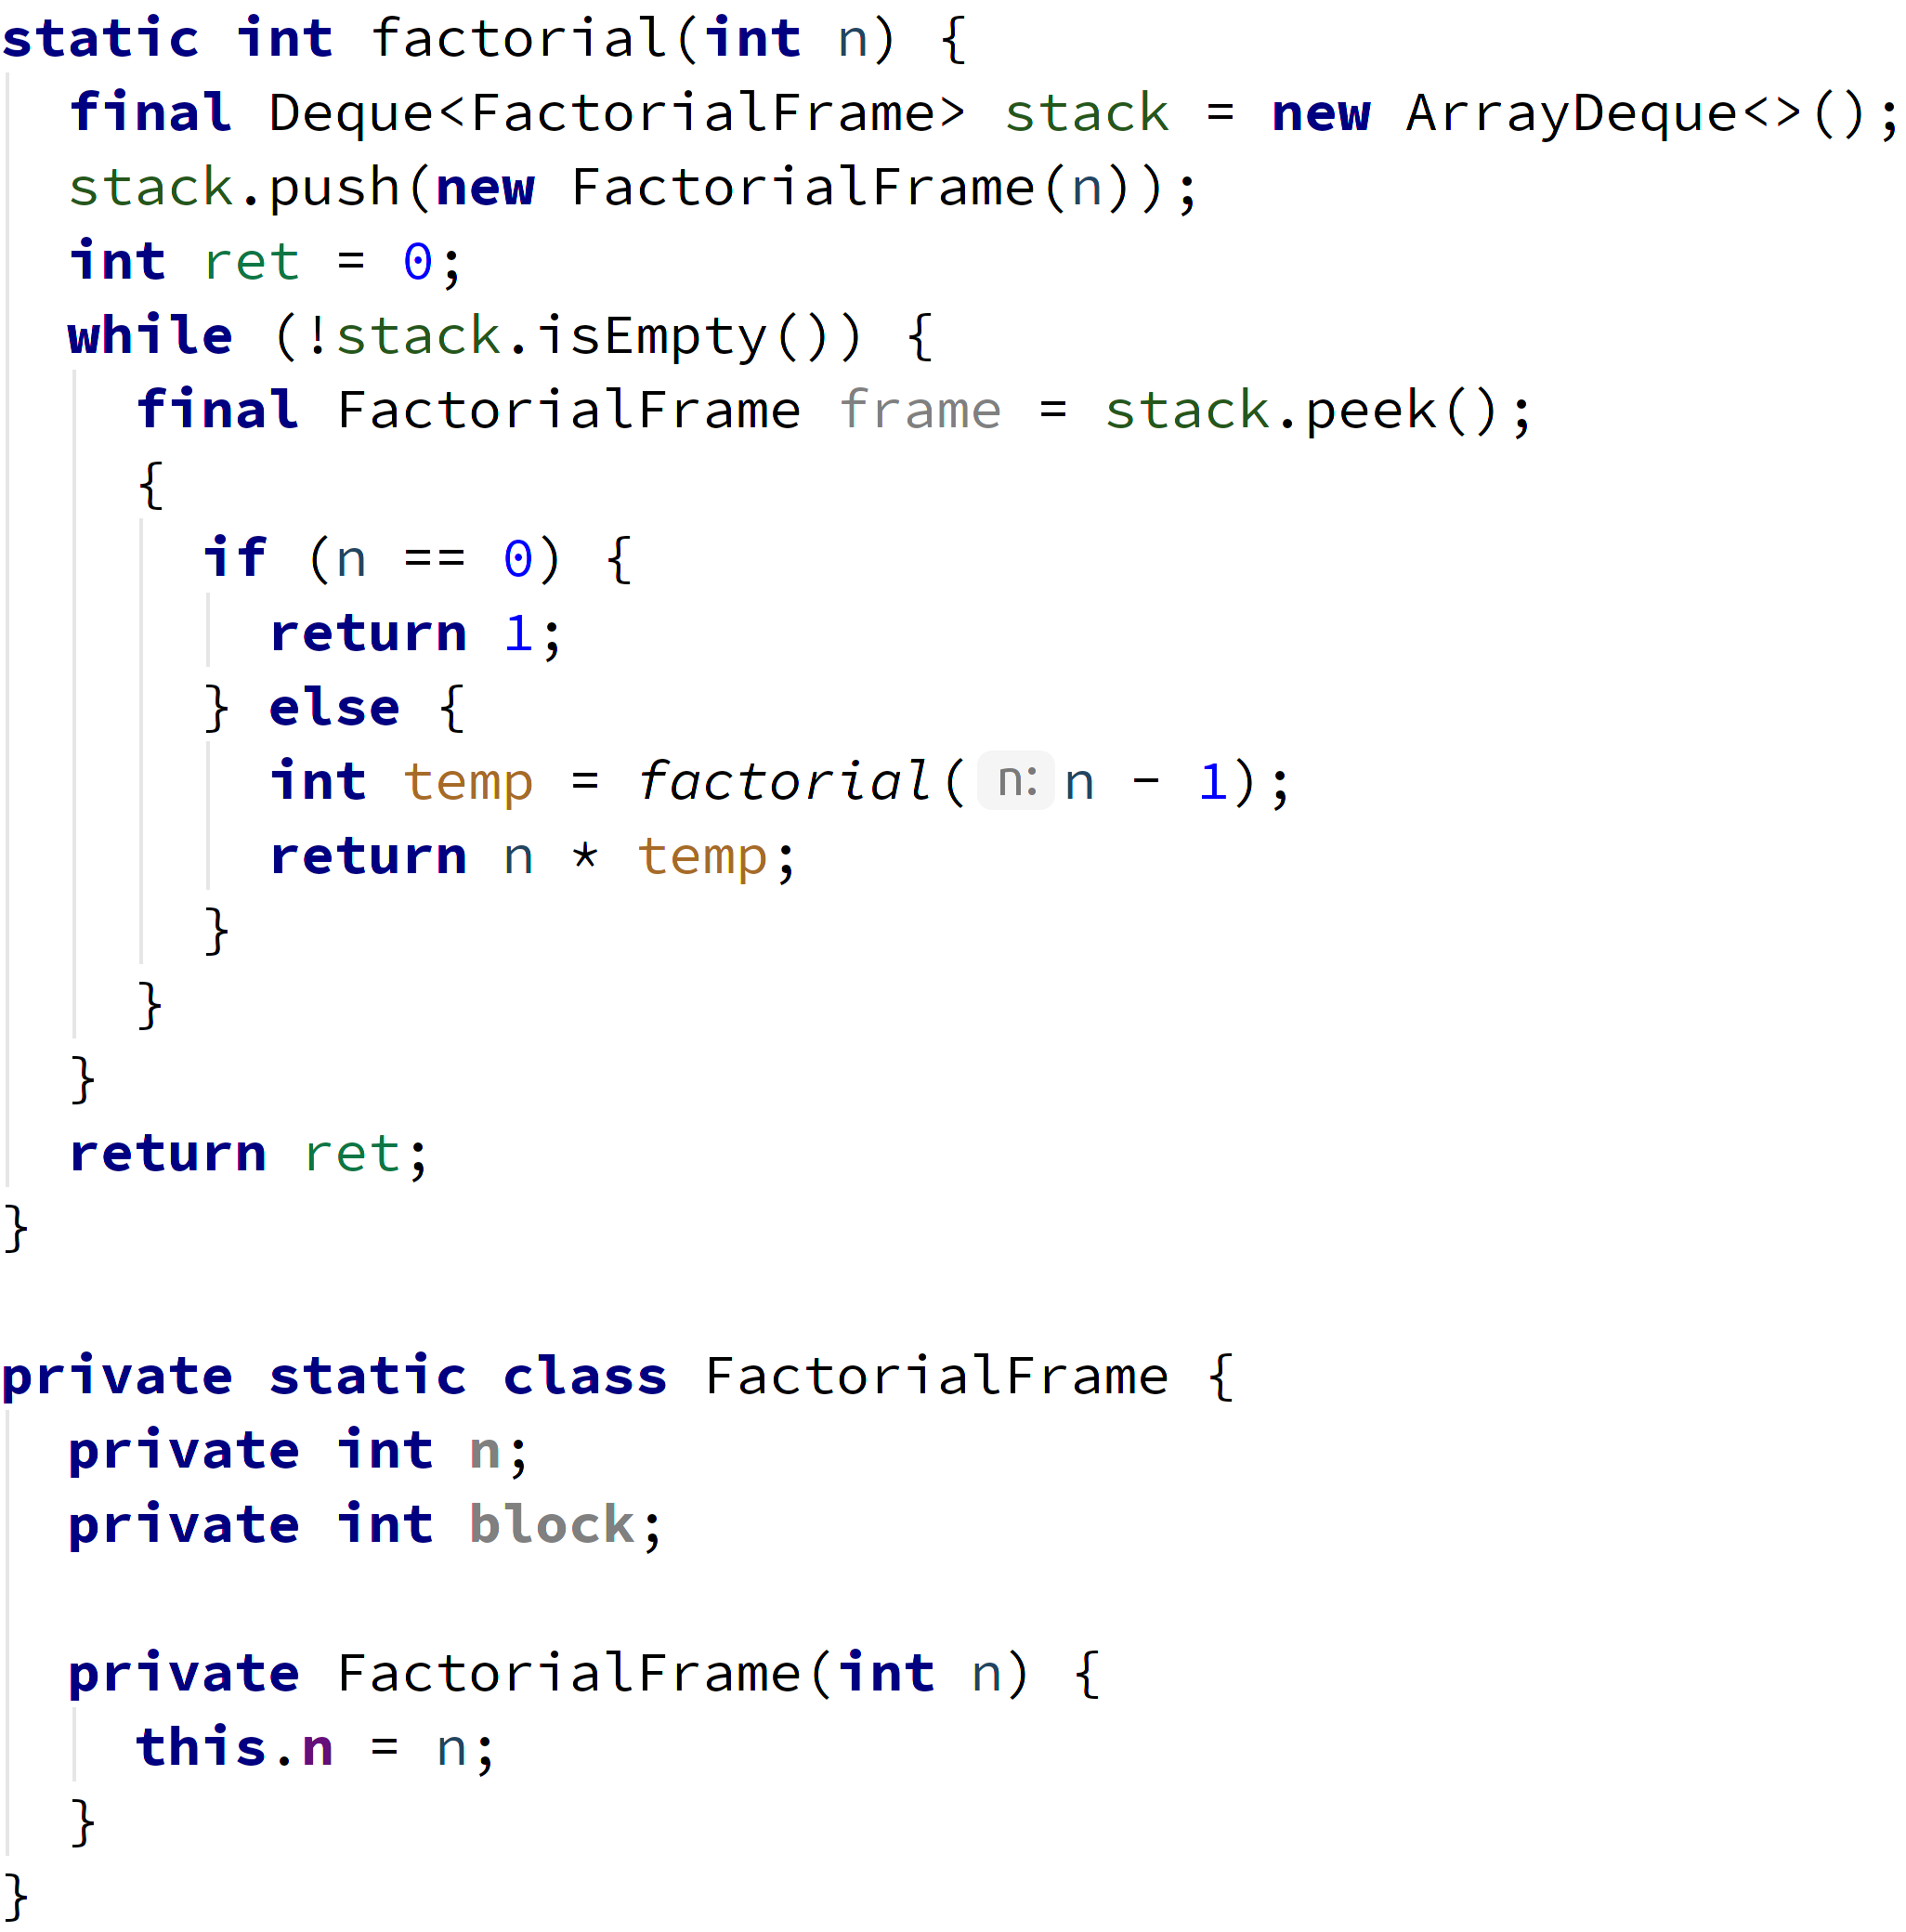
\includegraphics[height=2.456in]{../../../theses/diploma/src/img/incorporate-after-white-26.png}
            \caption{După}
        \end{subfigure}%
        }\\
        \caption{Includerea codului metodei în codul auxiliar}
    \end{figure}
\end{frame}

\begin{frame}{Înlocuirea referințelor la variable cu accese la câmpul din cadrul de stivă}
    \begin{figure}[htb]
        \makebox[\linewidth][c]{%
        \begin{subfigure}[b]{.5\textwidth}
            \centering
            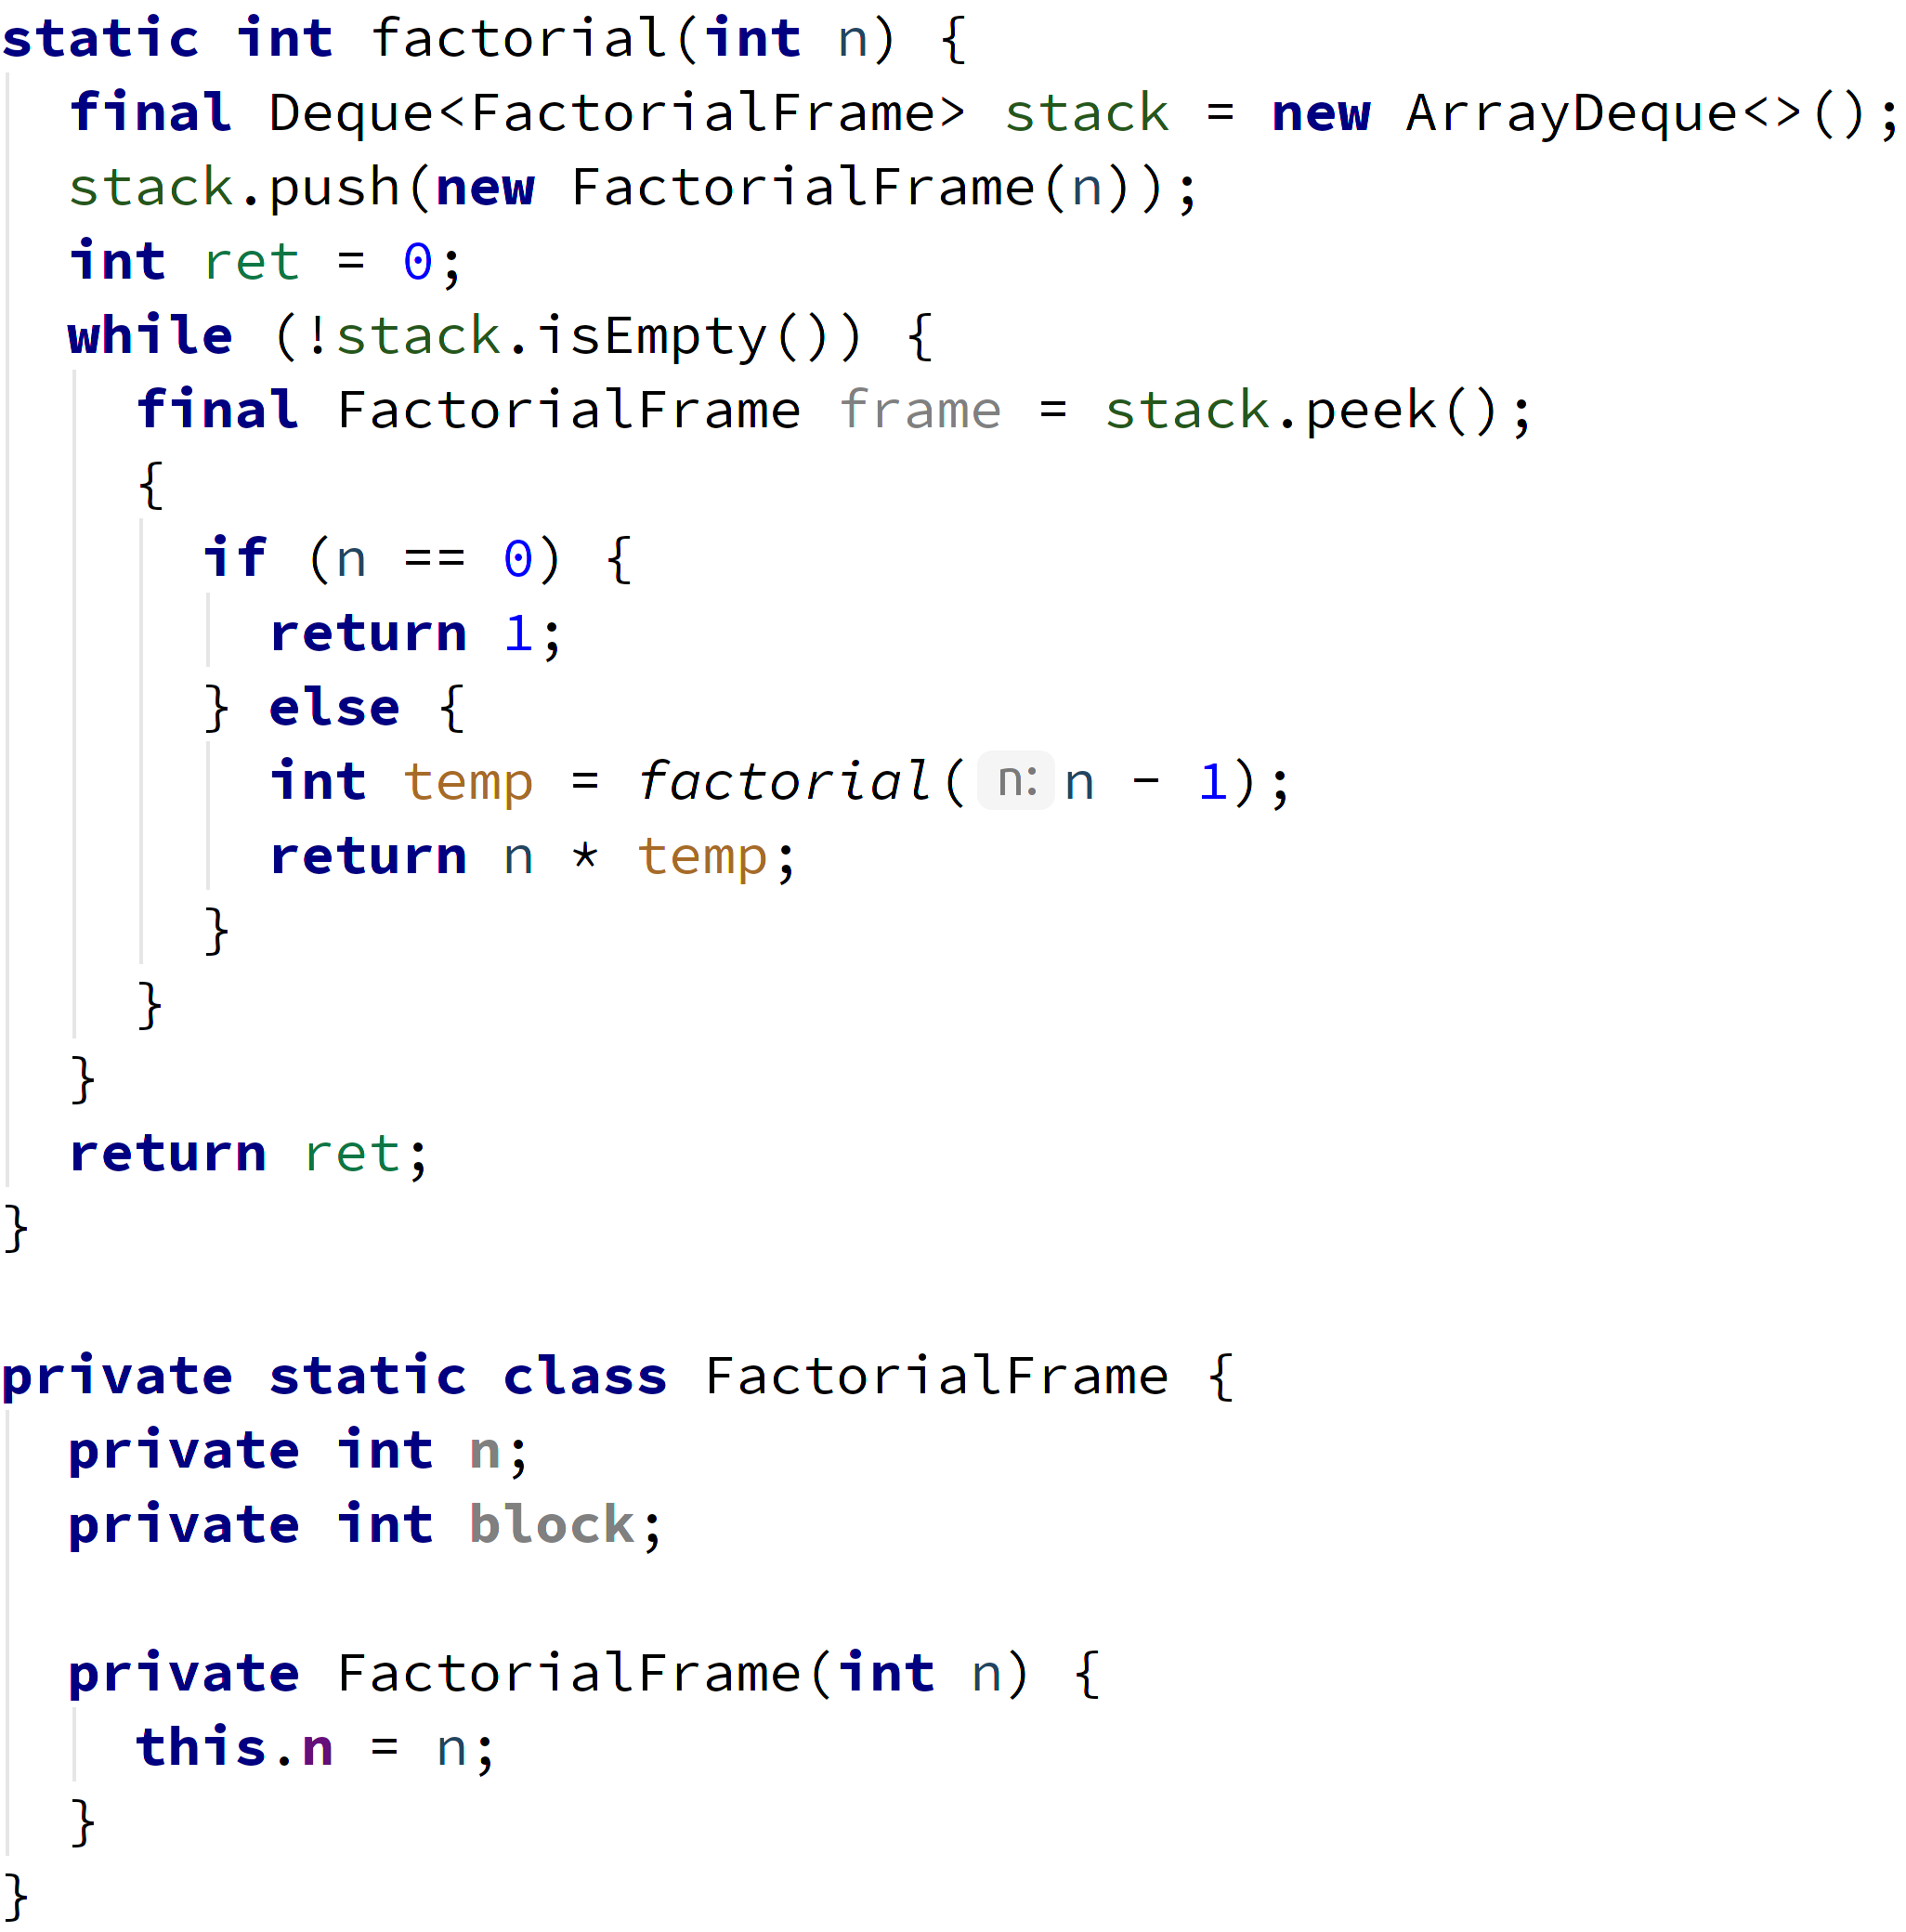
\includegraphics[width=2.1in]{../../../theses/diploma/src/img/incorporate-after-white-26.png}
            \caption{Înainte}
        \end{subfigure}%
        \begin{subfigure}[b]{.5\textwidth}
            \centering
            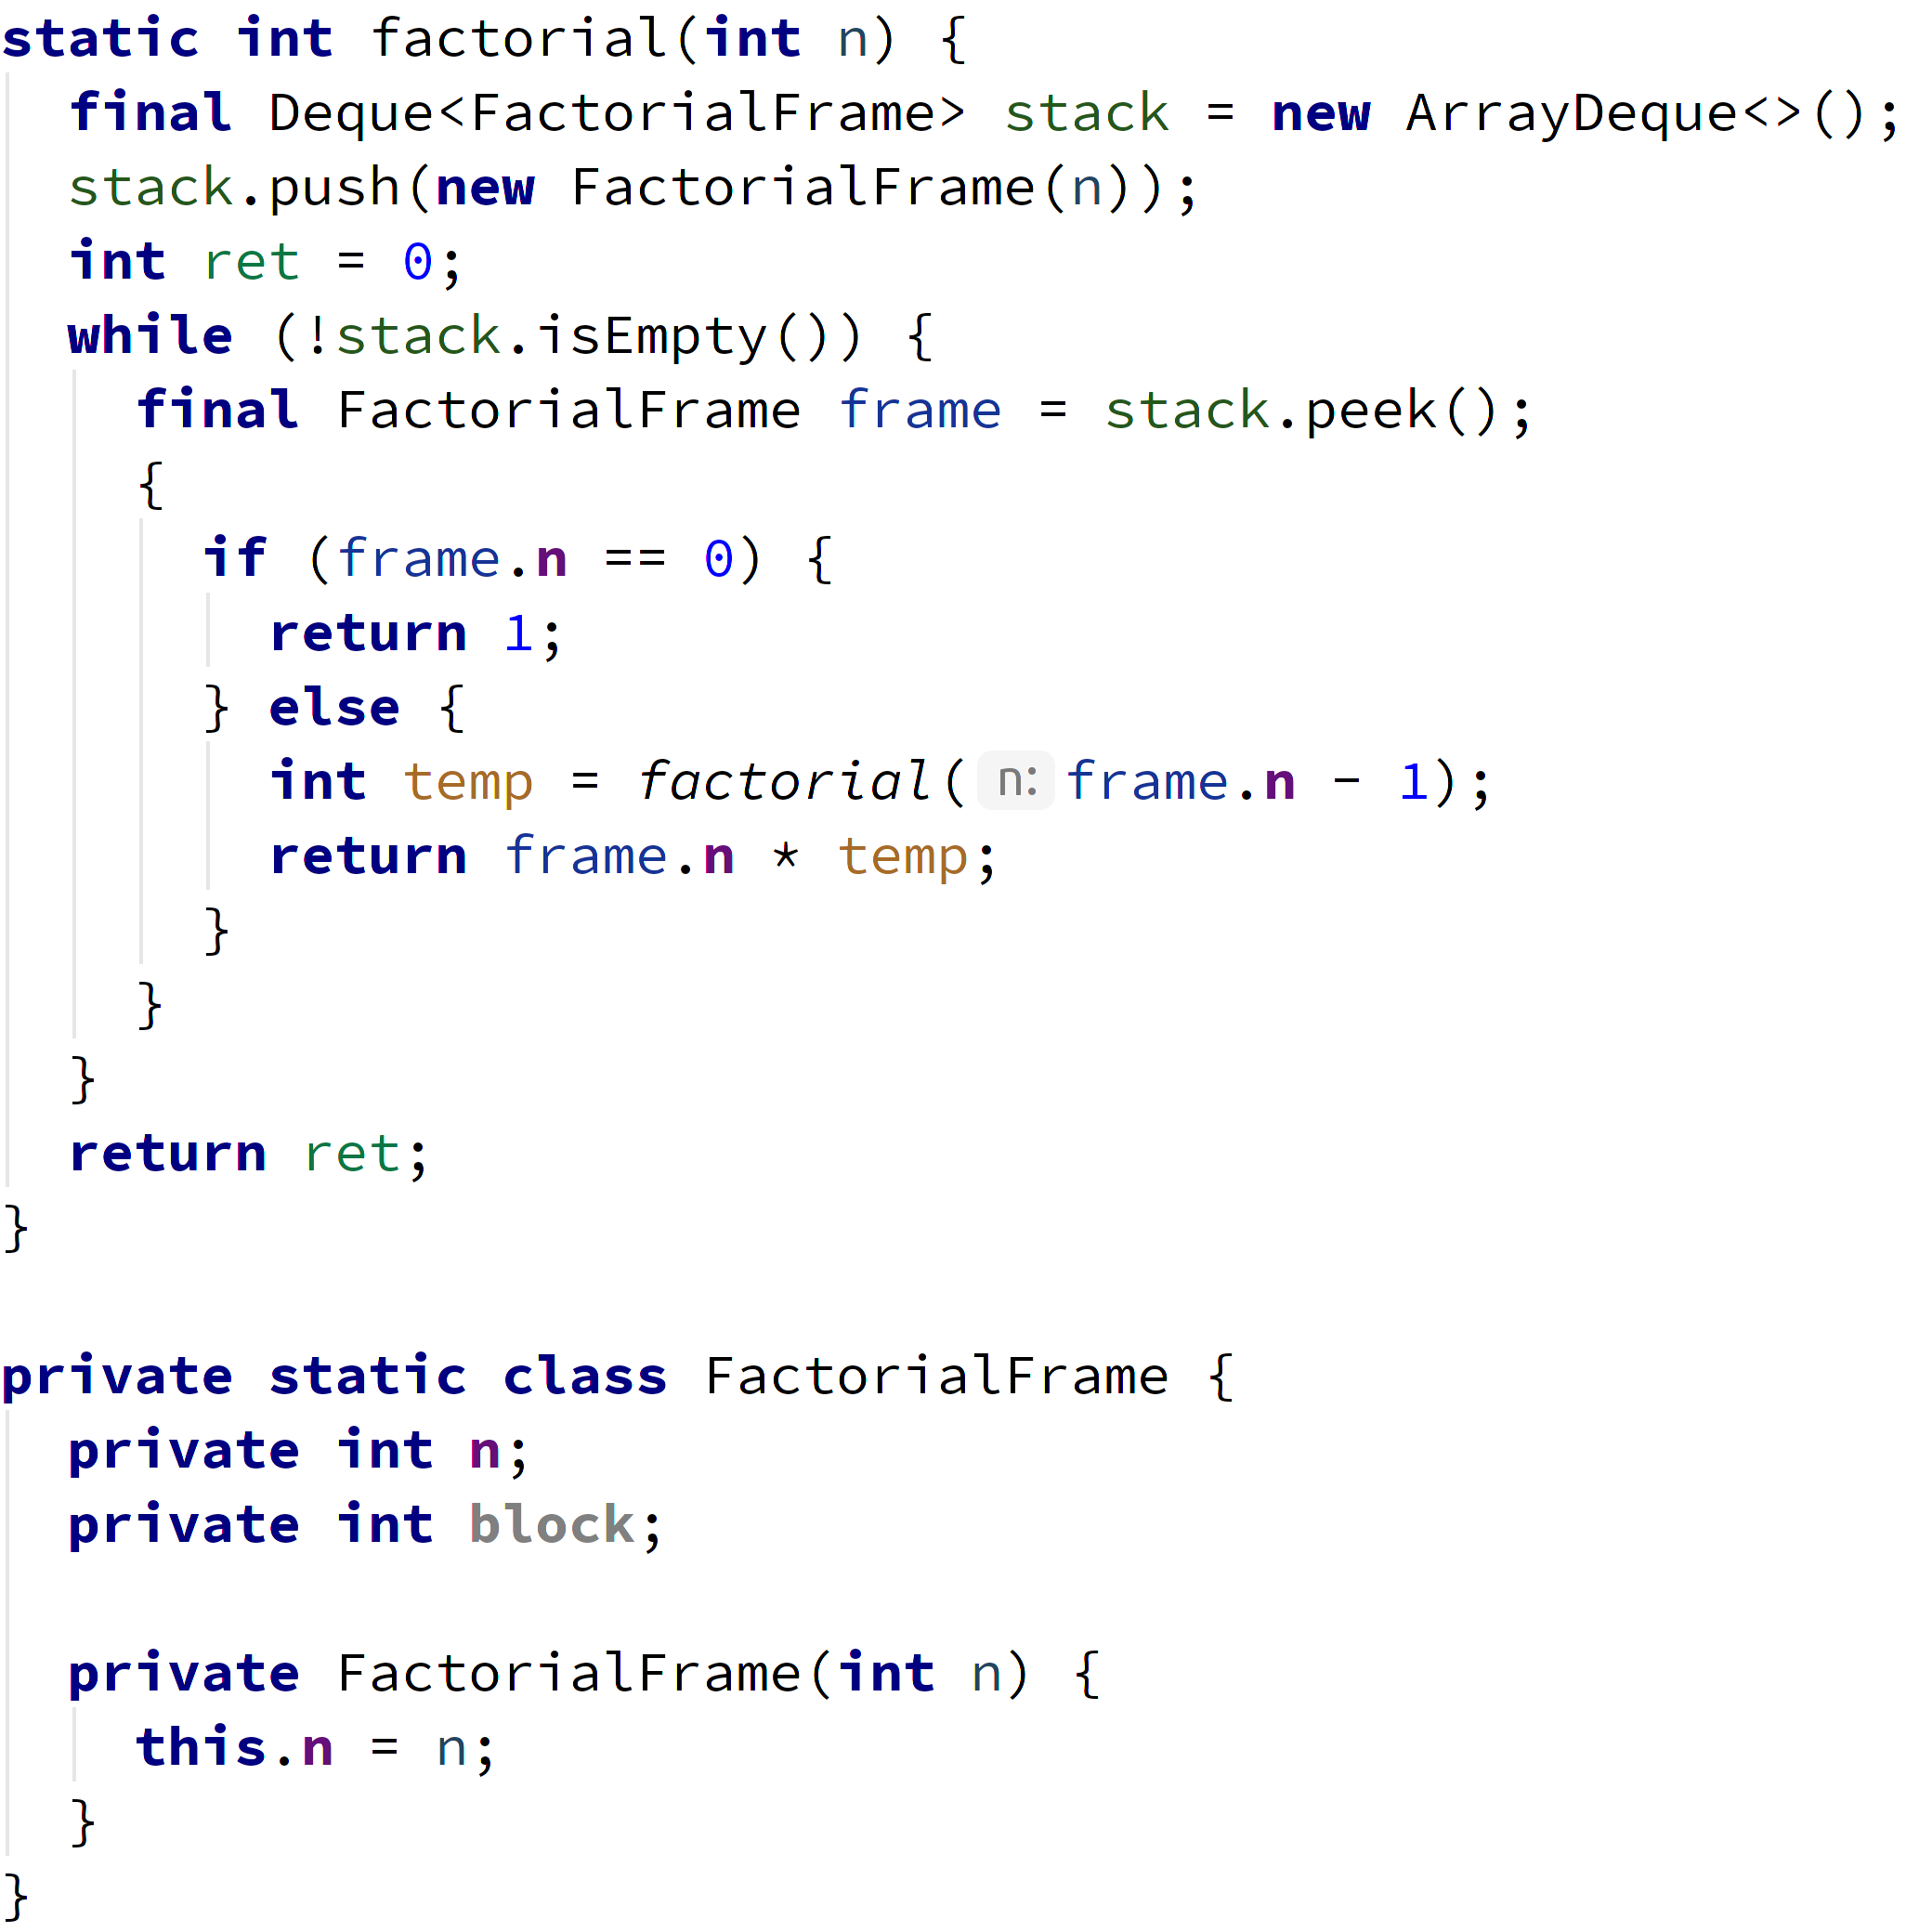
\includegraphics[width=2.1in]{../../../theses/diploma/src/img/ref-frame-after-white-26.png}
            \caption{După}
        \end{subfigure}%
        }\\
        \caption{Înlocuirea referințelor la variable cu accese la câmpul din cadrul de stivă}
    \end{figure}
\end{frame}

\begin{frame}{Înlocuirea declarațiilor având inițializare cu accese la câmpul din cadrul de stivă}
    \begin{figure}[htb]
        \makebox[\linewidth][c]{%
        \begin{subfigure}[b]{.5\textwidth}
            \centering
            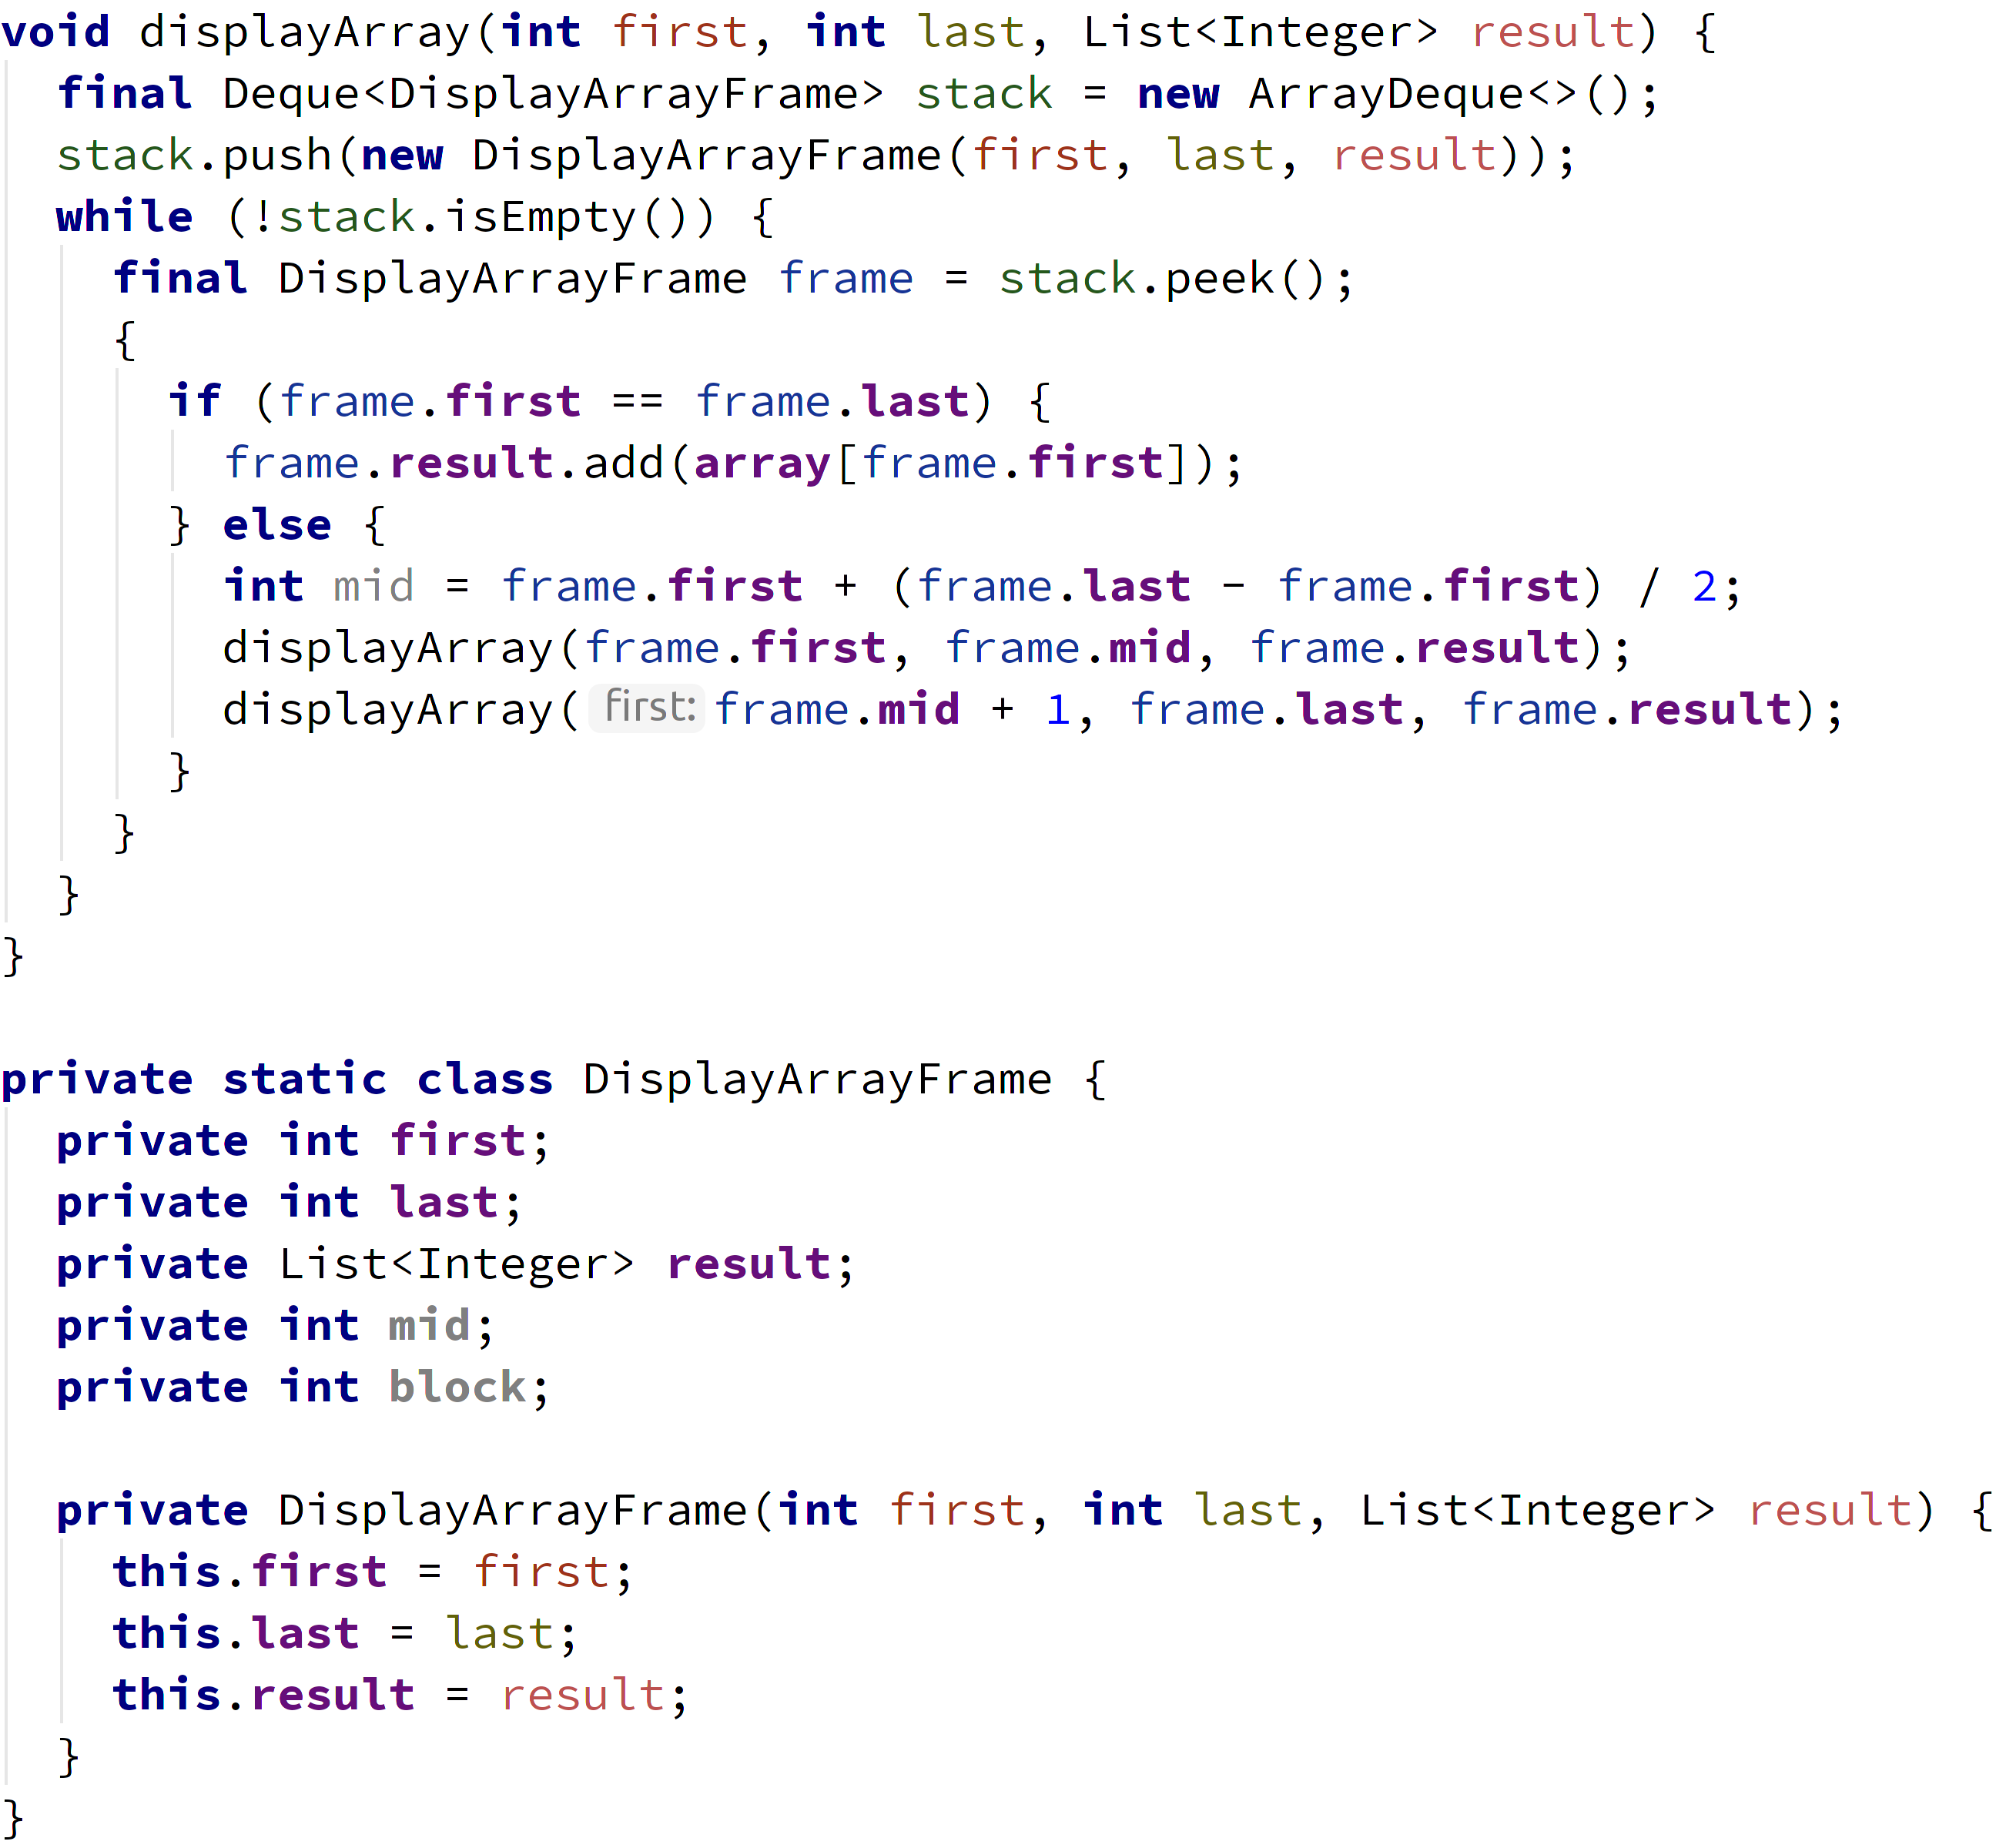
\includegraphics[width=2.1in]{../../../theses/diploma/src/img/replace-declaration-before-white-30.png}
            \caption{Before}
        \end{subfigure}%
        \begin{subfigure}[b]{.5\textwidth}
            \centering
            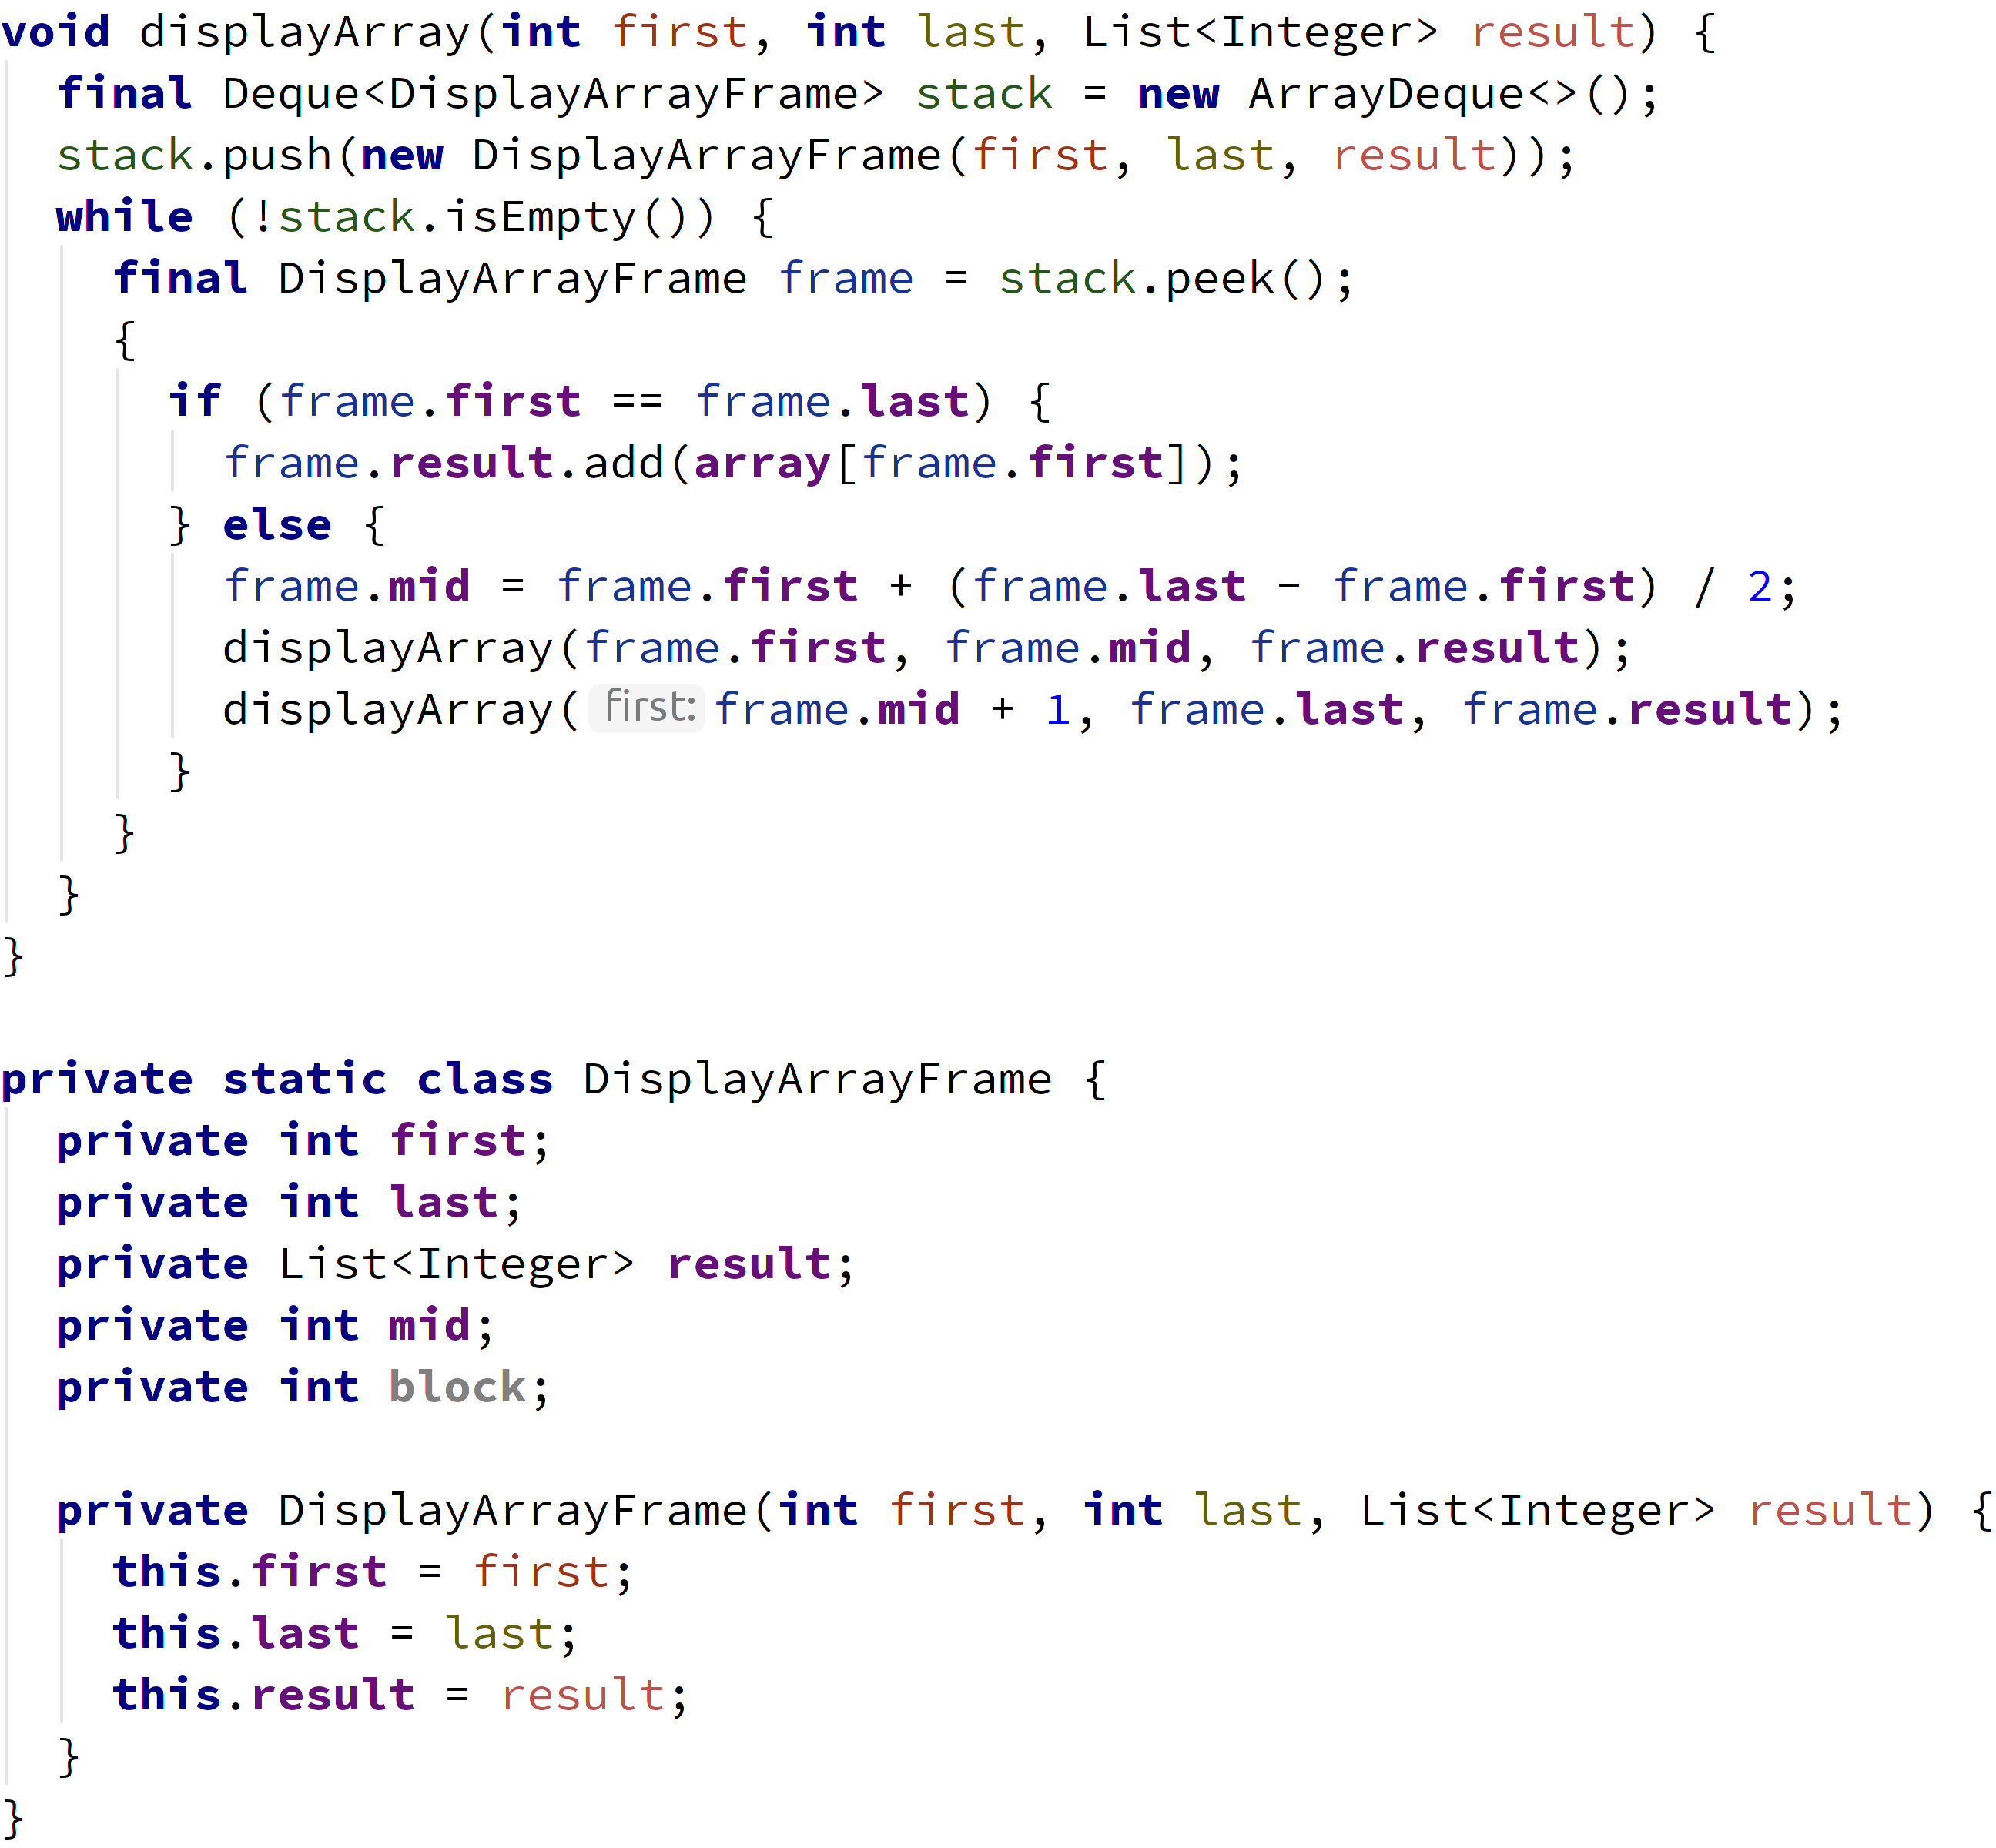
\includegraphics[width=2.1in]{../../../theses/diploma/src/img/replace-declaration-after-white-30.png}
            \caption{After}
        \end{subfigure}%
        }\\
    \end{figure}
\end{frame}

\begin{frame}{Generarea grafului fluxului de control (Instrucțiunea \code{if})}
    \begin{figure}[htb]
        \centering
        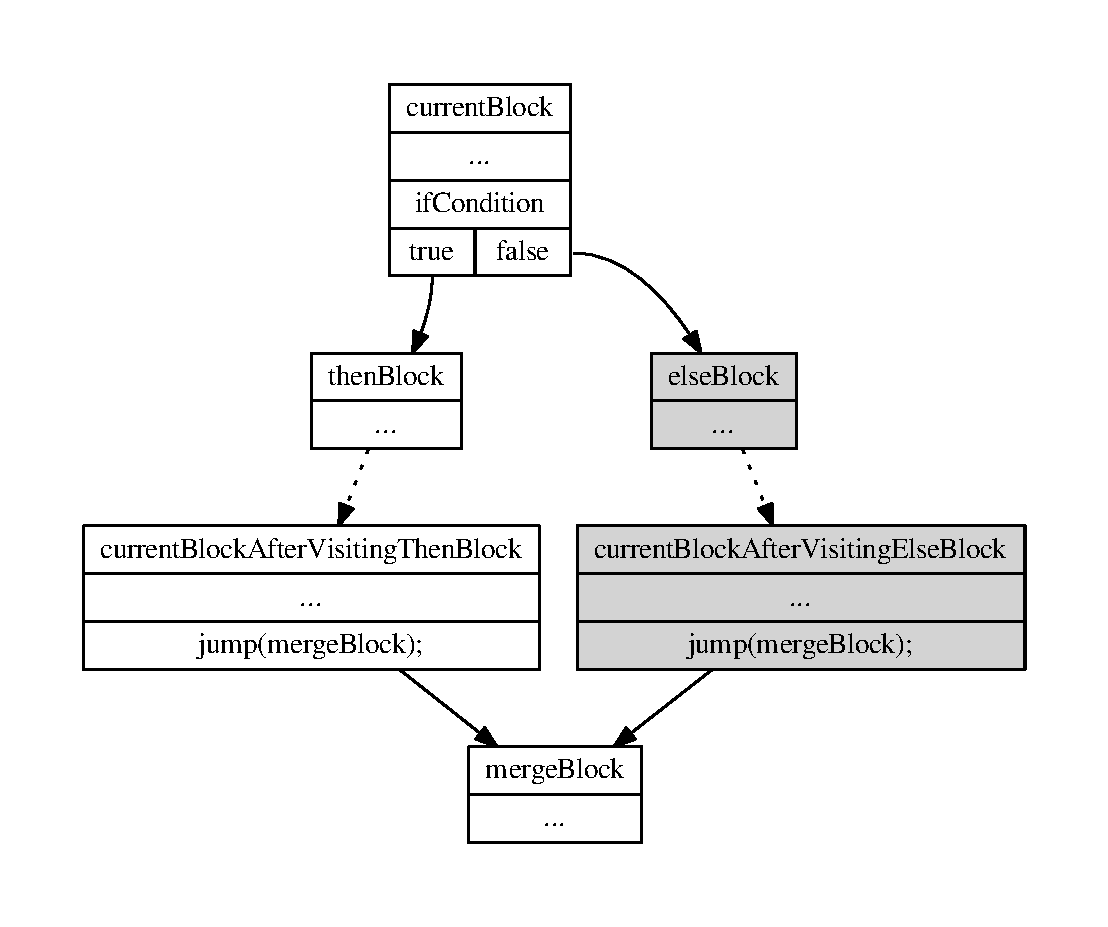
\includegraphics[width=.7\textwidth]{../../../theses/diploma/src/graph/if.pdf}
    \end{figure}
\end{frame}

\begin{frame}{Generarea grafului fluxului de control (Instrucțiuni de ciclare)}
    \begin{figure}[htb]
        \begin{subfigure}[b]{0.32\textwidth}
            \centering
            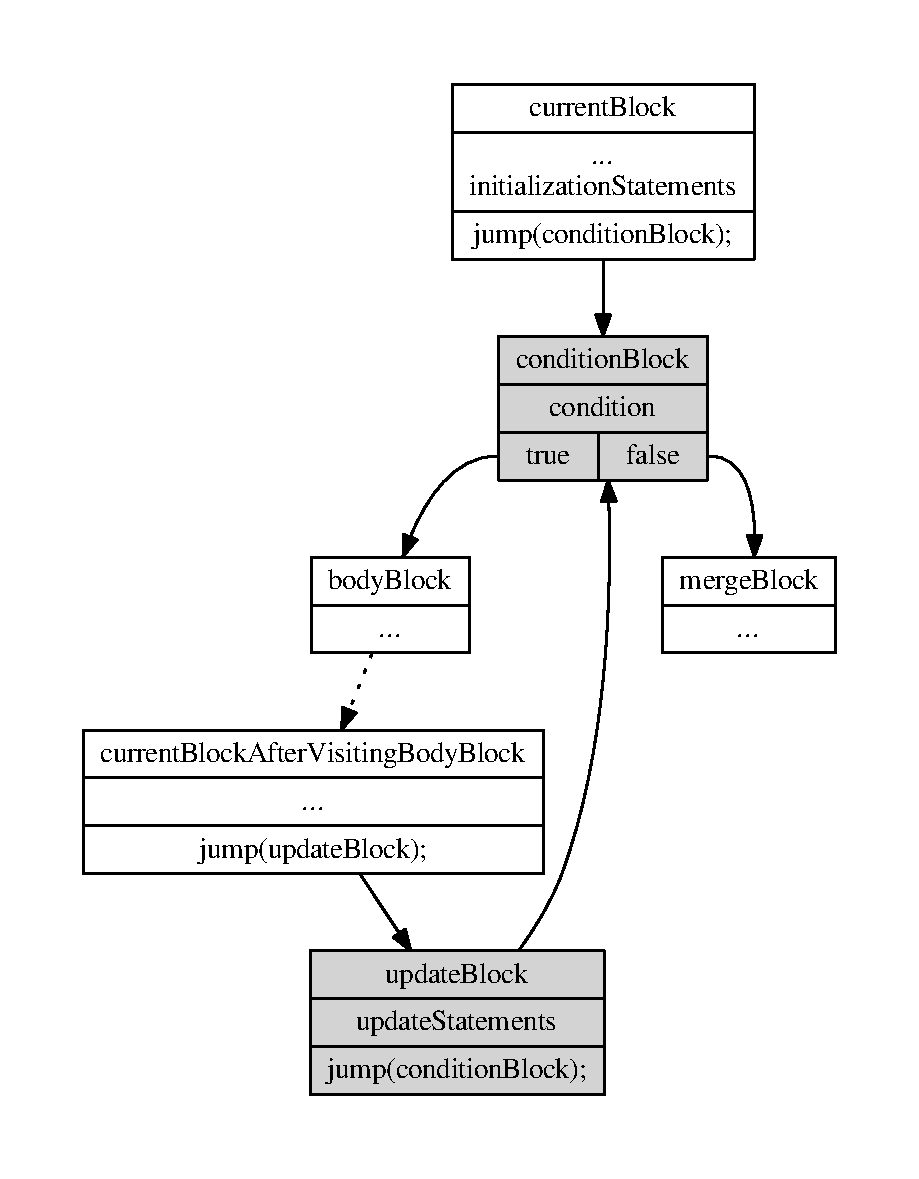
\includegraphics[width=\textwidth]{../../../theses/diploma/src/graph/for.pdf}
            \caption{\code{for}}
        \end{subfigure}
        \hfill
        \begin{subfigure}[b]{0.32\textwidth}
            \centering
            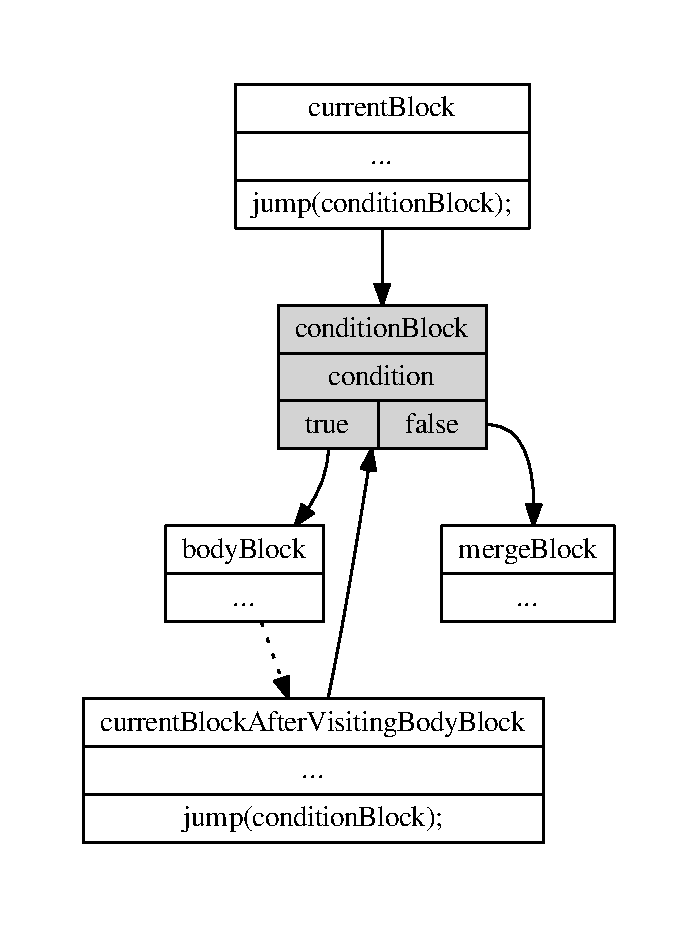
\includegraphics[width=\textwidth]{../../../theses/diploma/src/graph/while.pdf}
            \caption{\code{while}}
        \end{subfigure}
        \hfill
        \begin{subfigure}[b]{0.32\textwidth}
            \centering
            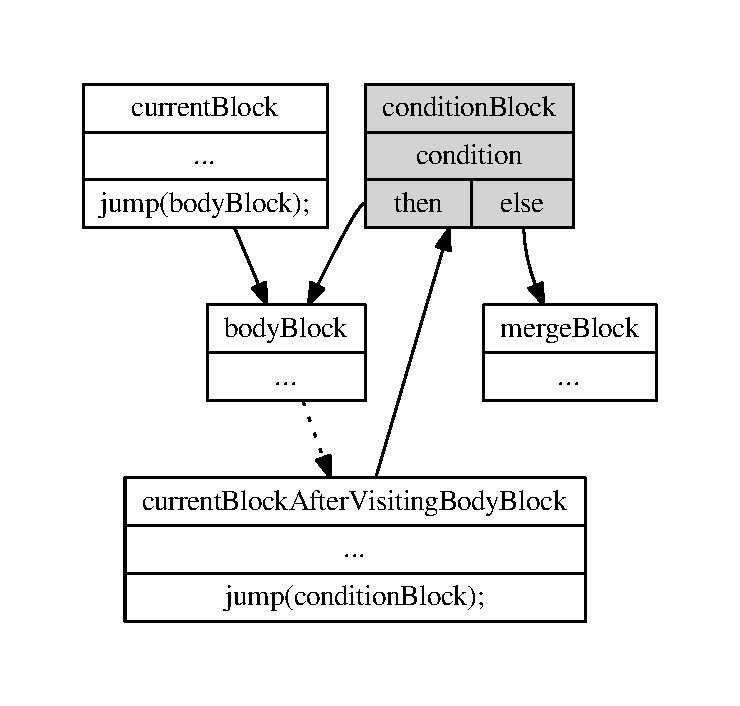
\includegraphics[width=\textwidth]{../../../theses/diploma/src/graph/do-while.pdf}
            \caption{\code{do-while}}
        \end{subfigure}
    \end{figure}
\end{frame}

\begin{frame}{Generarea grafului fluxului de control (Exemplu)}
    \begin{figure}[htb]
        \begin{subfigure}[b]{.4\textwidth}
            \centering
            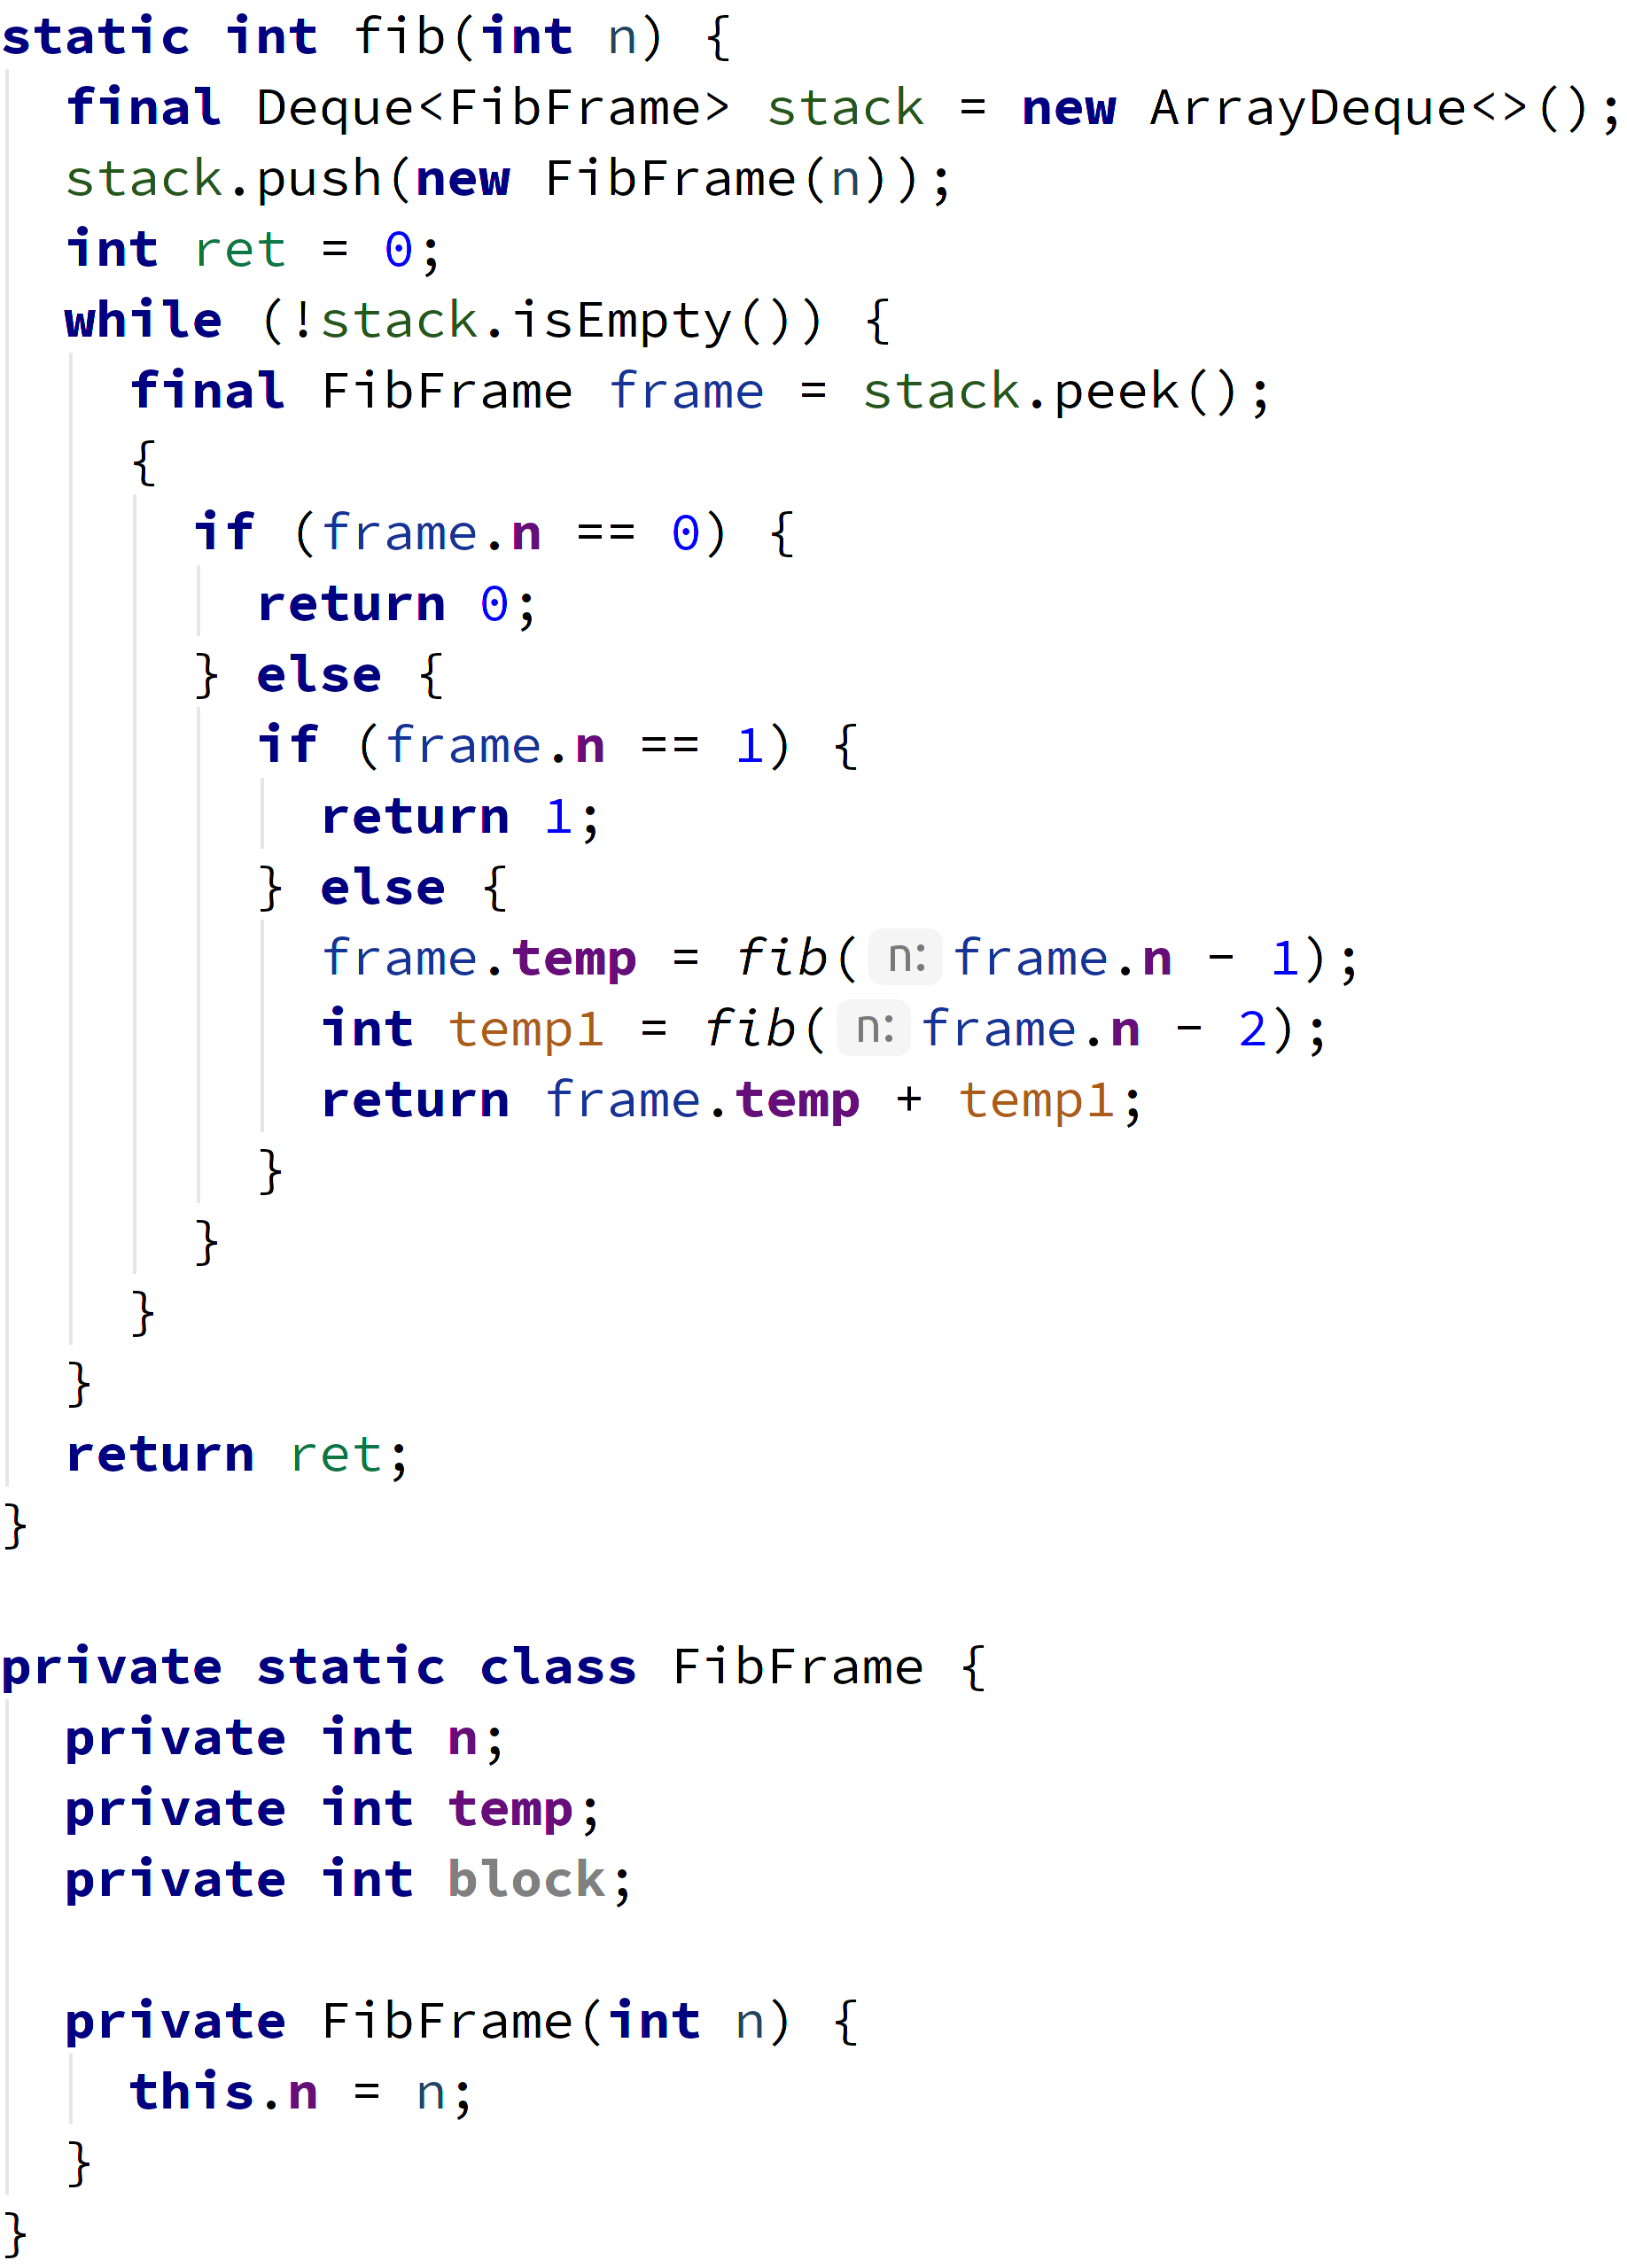
\includegraphics[width=\textwidth]{../../../theses/diploma/src/img/cfg-before-white-32.png}
        \end{subfigure}
        \begin{subfigure}[b]{.4\textwidth}
            \centering
            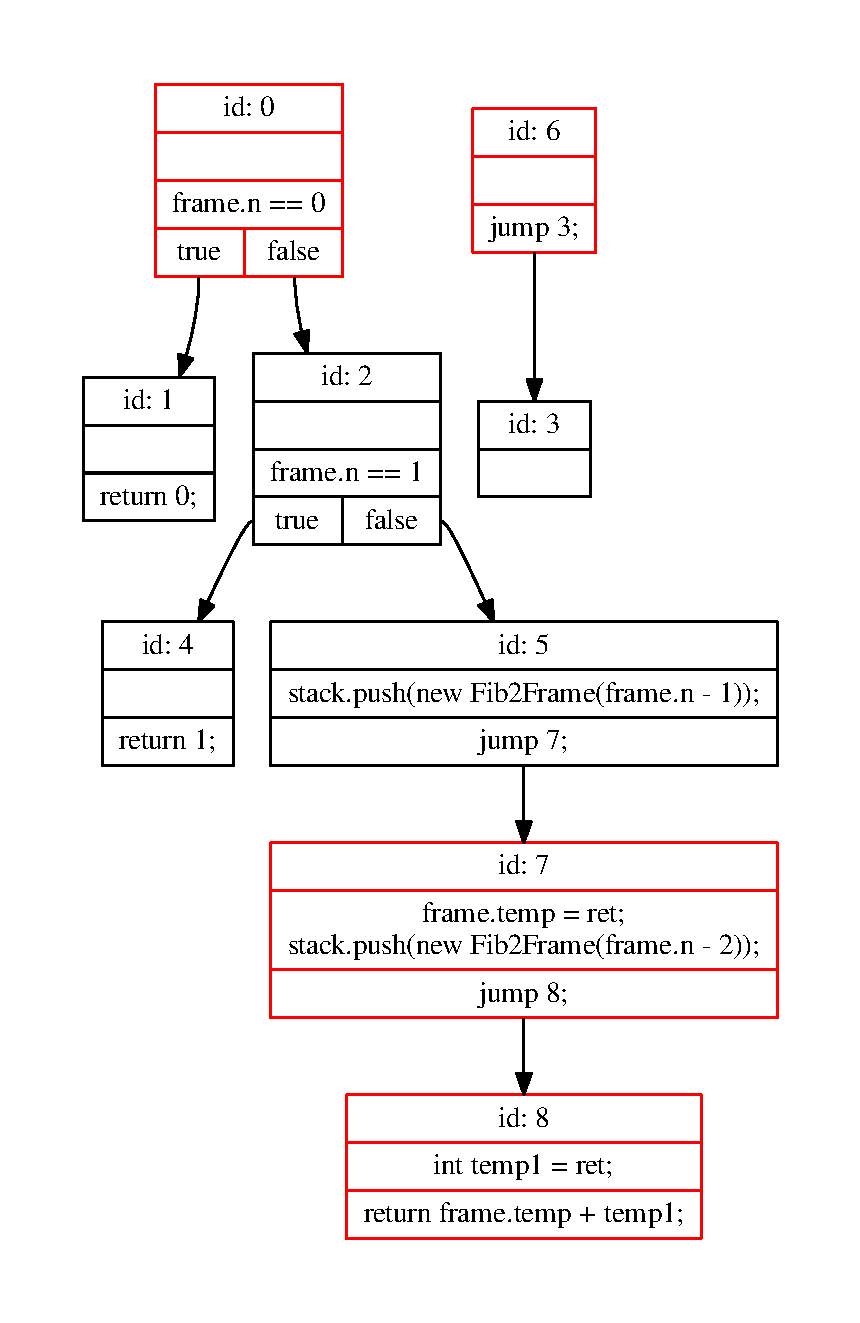
\includegraphics[width=\textwidth]{../../../theses/diploma/src/graph/cfg.pdf}
        \end{subfigure}
    \end{figure}
\end{frame}

\begin{frame}{Porțiuni de cod}
	\documentclass{propsoa.cs.pub.ro}

\title{Project Name}
\subtitle{Project Proposal, SOA/OS -- Autumn 2010}
\version{1.1/\today}
\indexterms{project scope}
\keywords{project/paper specific topics}
\teamsize{number of students in team}

\begin{document}
\maketitle

\section{Project Description}

The scientific context in which the project is developed must be presented.
The purpose and objective of the project must be properly stated.

\section{Objectives}

This project aims to implement a software application that will meet the
following requirements:
\begin{itemize}
	\item{Objective 1}
	\item{Objective 2}
	\item{Objective 3}
\end{itemize}

\section{Bibliography}

list of papers, books, links

\section{Prerequisites}

Fields of study, technologies.

\section{Other}

(other useful information, etc. --- section may be missing)

\end{document}

\end{frame}
	
\section{Rezultate}

\begin{frame}{TODO}
	\begin{itemize}
		\item TODO
		\item TODO
	\end{itemize}
\end{frame}

\section{\^{I}ntrebări}

\begin{frame}{Întrebări}
  \begin{columns}
    \begin{column}[t]{0.5\textwidth}
      \begin{itemize}
        \item cuvânt cheie 1
        \item cuvânt cheie 2
        \item cuvânt cheie 3
        \item cuvânt cheie 4
        \item cuvânt cheie 5
      \end{itemize}
    \end{column}
    \begin{column}[c]{0.5\textwidth}
      \begin{figure}
        
\includegraphics[scale=0.3]{img/question-mark}
      \end{figure}
    \end{column}
  \end{columns}
\end{frame}

\end{document}
